\documentclass[times, utf8, zavrsni]{fer}
\usepackage{booktabs}
\usepackage[hidelinks]{hyperref}
\usepackage{listings}
\usepackage{multicol}
\usepackage{caption}
\usepackage{subcaption}

\graphicspath{ {./images/} }

\begin{document}

% TODO: Navedite broj rada.
\thesisnumber{448}

% TODO: Navedite naslov rada.
\title{Mobilna aplikacija za upravljanje receptima}

% TODO: Navedite vaše ime i prezime.
\author{Marko Tunjić}

\maketitle

% Dodavanje zahvale ili prazne stranice. Ako ne želite dodati zahvalu, naredbu ostavite radi prazne stranice.
\zahvala{}

\tableofcontents

\chapter{Uvod}
Internet i web stranice su već dugo vremena dio ljudske svakodnevice no zbog
današnje potrebe za brzinom i efikasnošću sve popularnije su mobilne aplikacije. Naime one
su vrlo jednostavne za koristiti jer je potrebno samo izvaditi mobitel
kliknuti na aplikaciju i sve je spremno. Upravo zato danas puno web aplikacija
također ima i svoju mobilnu inačicu.
\\\\
Tako se do danas pojavio velik broj jezika
i radnih okvira za razvoj mobilnih aplikacija kao na primjer kotlin, swift, flutter,
react native i slično. Problem kod mobilnih uređaja je što ovisno koji operacijski
sustav uređaj koristi jedna aplikacija neće biti kompatibilna na svim ostalima.
Neki od prethodno navedenih radnih okvira, kao na primjer: flutter i react native,
rješavaju problem kompatibilnosti operacijskih sustava uređaja takozvanim \textit{"native"} pristupom
i jednom isprogramirana aplikacija u tim okvirima će se moći izvoditi na svim uređajima.
\\\\
Unatoč tranziciji sa preglednika na mobilne uređaje nije nestala potreba
za poslužiteljskim dijelom i bazom podataka, jer takva arhitektura omogućava
komunikaciju i dijeljenje sadržaja među ljudima širom svijeta. Pa se tako na
poslužiteljskoj strani i dalje koriste stvari kao Spring, ASP.NET i slični okviri,
a za bazu podataka upravitelji po izboru na primjer PostgreSQL, MSSQL, MySQL\dots
Iz tog razloga je još uvijek popularan oblikovni obrazac MVC (Model-View-Controller).
\\\\
Radi jednostavnosti se mobilne aplikacije ne koriste starijim protokolima kao na primjer
SOAP i XML formatom podatka nego se koriste novijim načinom prijenosa
podataka između poslužiteljskog dijela aplikacije i korisničkog dijela aplikacije.
To je JSON format podataka s odgovarajućim JSON zahtjevima prema poslužitelju.
Uz JSON se koristi neki od arhitekturnih stilova kao REST ili GraphQL koji su alternativa
za SOAP protokol i s njime mogu i web i mobilne aplikacije uspješno i jednostavno uspostavljati komunikaciju.
\\\\
Također zbog naglog razvoja interneta i pojave velikog broja poslužitelja i baza podataka
pojavila se potreba za računalima na kojima će biti pokrenuti ti poslužitelji i
baze podataka, tako se pojavio \textit{"oblak"} i usluge u oblaku \textit{(eng. Cloud, Cloud Services)}.
Uz pomoć tih usluga vrlo je lako pokrenuti instancu potrebne baze i poslužitelja
u \textit{"oblaku"} koji će biti globalno dostupan. Kao pružatelji takvih usluga ističu se:
AWS, Heroku, Azure i tako dalje.
\\\\
Cilj ovoga rada bio je izraditi mobilnu aplikaciju koja će korisnicima olakšati: pristup,
pamćenje, dijeljenje i pretraživanje recepata. Sadržaj je podijeljen u 4 dijela u kojima
će se opisati zahtjevi, način izrade svakog sloja aplikacije (baza podataka,
poslužiteljski i korisnički dio), korištene tehnologije i konačni proizvod.

\chapter{Zahtjevi}

\section{Funkcionalni}
\begin{enumerate}
      \item \textbf{\underline{Korisnici aplikacije:}} Aplikaciji mogu pristupiti 3 vrste korisnika:
            anonimni, prijavljeni i administratori, a ovisno o vrsti korisnika kojoj pripada, svaki korisnik ima
            različite ovlasti i uloge.
      \item \textbf{\underline{Mogućnosti anonimnih korisnika:}} oni mogu samo pregledavati i pretraživati
            recepte. Recepti se mogu pretraživati po nazivu ili po sastojcima pri čemu se pretraga po
            sastojcima može obaviti po sastojcima koje recept ne smije sadržavati (što je bitno zbog
            alergija) ili po sastojcima koje korisnik ima pri ruci.
      \item \textbf{\underline{Mogućnosti prijavljenih korisnika:}} prijavljeni korisnici uz funkcionalnosti \linebreak
            anonimnih korisnika mogu također i dodavati vlastite recepte, komentirati sve recepte
            i dodavati željene recepte u listu omiljenih recepata pri čemu korisnik na vlastiti e-mail
            dobije poruku s listom potrebnih sastojaka koja može poslužiti kao lista za kupnju.
      \item \textbf{\underline{Mogućnosti administratora:}} administratori za razliku od prijavljenih
            korisnika ne mogu dodavati vlastite recepte, ali zato imaju ulogu odobravanja recepata, jer
            naime prije negoli bilo koji recept postane javno vidljiv administratori ga moraju odobriti.
      \item \textbf{\underline{Format recepta:}} uz zahtjeve da recept ima svoje korake pripreme i
            sastojke potrebne za izradu jela, svaki recept također može imati priloženo više fotografija
            i/ili videozapisa koji pobliže opisuju recept i pomažu korisnicima pri kuhanju.
      \item \textbf{\underline{Registracija:}} korisnik će pri registraciji morati predati neku vlastitu
            postojeću e-mail adresu na koju će primati liste za kupnju od recepata koje dodaju u svoje favorite.
\end{enumerate}

\section{Dodatne funkcionalnosti}
\begin{enumerate}
      \item \textbf{\underline{Dodatne mogućnosti prijavljenih korisnika:}} prijavljeni korisnici će
            dodatno moći brisati vlastite recepte, komentare na vlastitim receptima i vlastite komentare
            na tuđim receptima. Također će moći ocjenjivati recepte ocjenama od 0 do 5 i pretraživati
            recepte po trajanju pripreme.
      \item \textbf{\underline{Dodatne mogućnosti administratora:}} administratori osim što mogu odobriti
            recepte isto tako ih mogu poništiti, nadalje mogu brisati sve recepte i sve komentare sa svih recepata
            i za kraj mogu suspendirati korisnike aplikacije \textit{(eng. ban)}.
      \item \textbf{\underline{Dodatni uvjeti:}} duljina raznih podataka koje korisnik šalje će biti
            određena dizajnom baze podataka, a veličina fotografija i videozapisa će biti određena
            HTTP poslužiteljem.
\end{enumerate}
\chapter{Baza podataka}
Kao upravitelj bazom podataka korišten je PostgreSQL i u svrhu lakšeg razvoja također
je korištena aplikacija sa korisničkim sučeljem za izvođenje upita: PgAdmin.
Sama baza je relacijskog tipa i modelirana je entitetima i vezama između njih.
Za modeliranje je korišten web alat ERDPlus. Za upogonjavanje baze je korišten \textit{AWS (Amazon Web Services)}
točnije njihov \textit{RDS (Relational Database Service)} servis koji se koristi upravo za upogonjavanje baza podataka u oblaku.

\section{Entiteti}
Entiteti su modelirani prema zahtjevima zadatka, a veze su modelirane prema stvarnim situacijama.
Postojeći entiteti su: recept, sastojak, korak pripreme, korisnik, uloga, videozapis i
fotografija. Dakle postoji glavni entitet koji je središte aplikacije, a to je recept
njega opisuju njegov identifikacijski broj, ime, opis, trajanje pripreme
te na kraju parametar koji pokazuje je li recept odobren od strane administratora ili nije.
Nadalje recept ne bi imao smisla da nema svoje korake pripreme i potrebne sastojke.
Također postoje fotografije i videozapisi jer svaki recept može imati
više videozapisa ili fotografija koji će uređivati korisničko sučelje
i pomoći korisnicima pri odabiru prikladnog recepta.
Korisnici su također modelirani kao jedan od entiteta jer mogu interagirati sa receptima
na razne načine, a te interakcije su opisane vezama kao što su komentiranje,
dodavanje u favorite, ocjenjivanje\dots Slika modela \textit{(eng. Entity relationship diagram)}
je prikazana na slici \ref{fig:ER Diagram}

\begin{figure}
      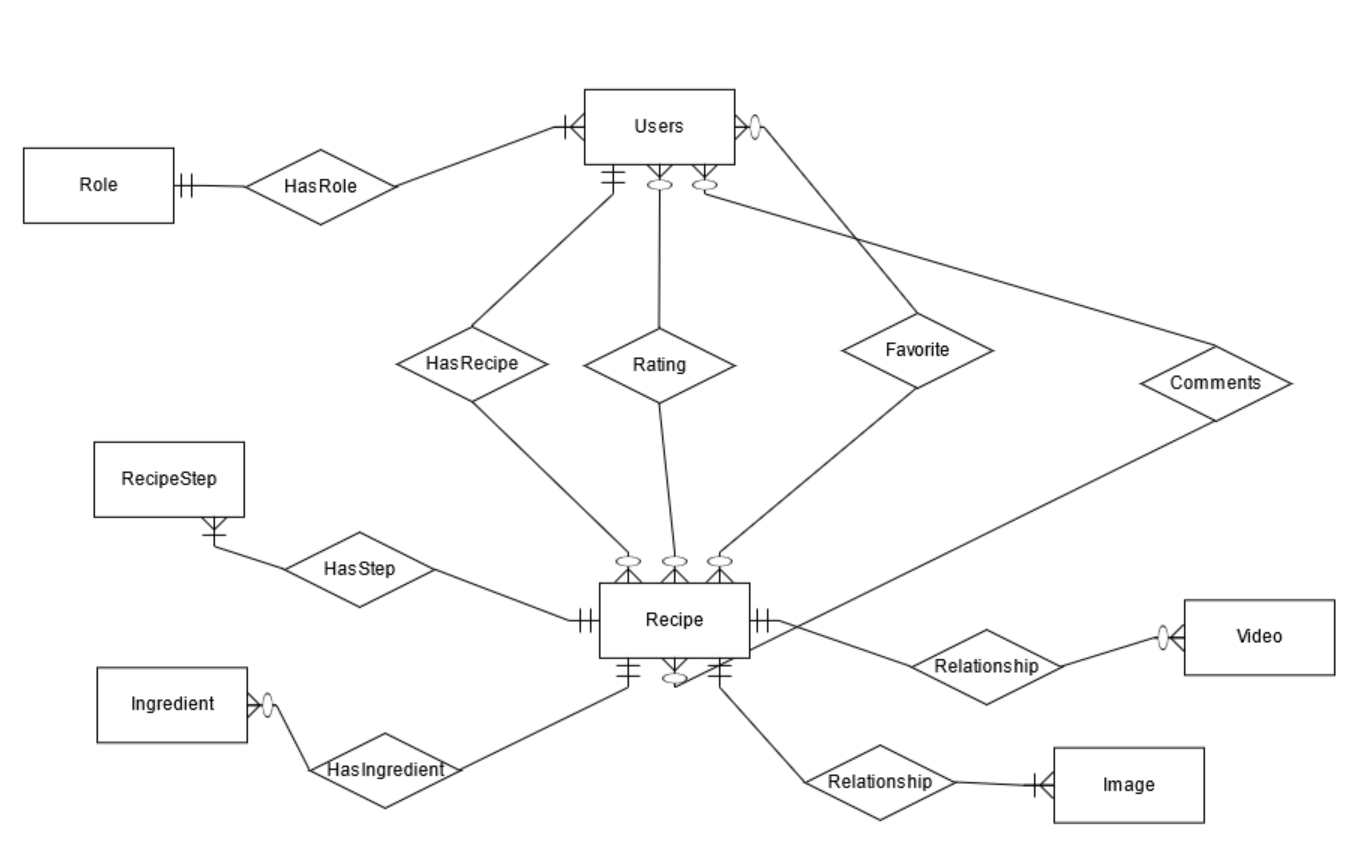
\includegraphics[width=\textwidth]{ERDiagram.png}
      \caption{ERDiagram}
      \label{fig:ER Diagram}
\end{figure}

\section{Relacije}
Iz prethodno opisanog modela pretvorbom iz entiteta u relacijsku shemu dobiveno je 10
tablica. One odgovaraju
entitetima i vezama između njih, tako se pojavljuju nove tablice koje predstavljaju:
komentare, favorite i ocjene. Dobivene tablice su stvorene u oblaku na upogonjenoj bazi.
Relacijska shema je prikaza slikom \ref{fig:Relacijska shema} i kodom \ref{lst:SQL kod}.

\begin{figure}
      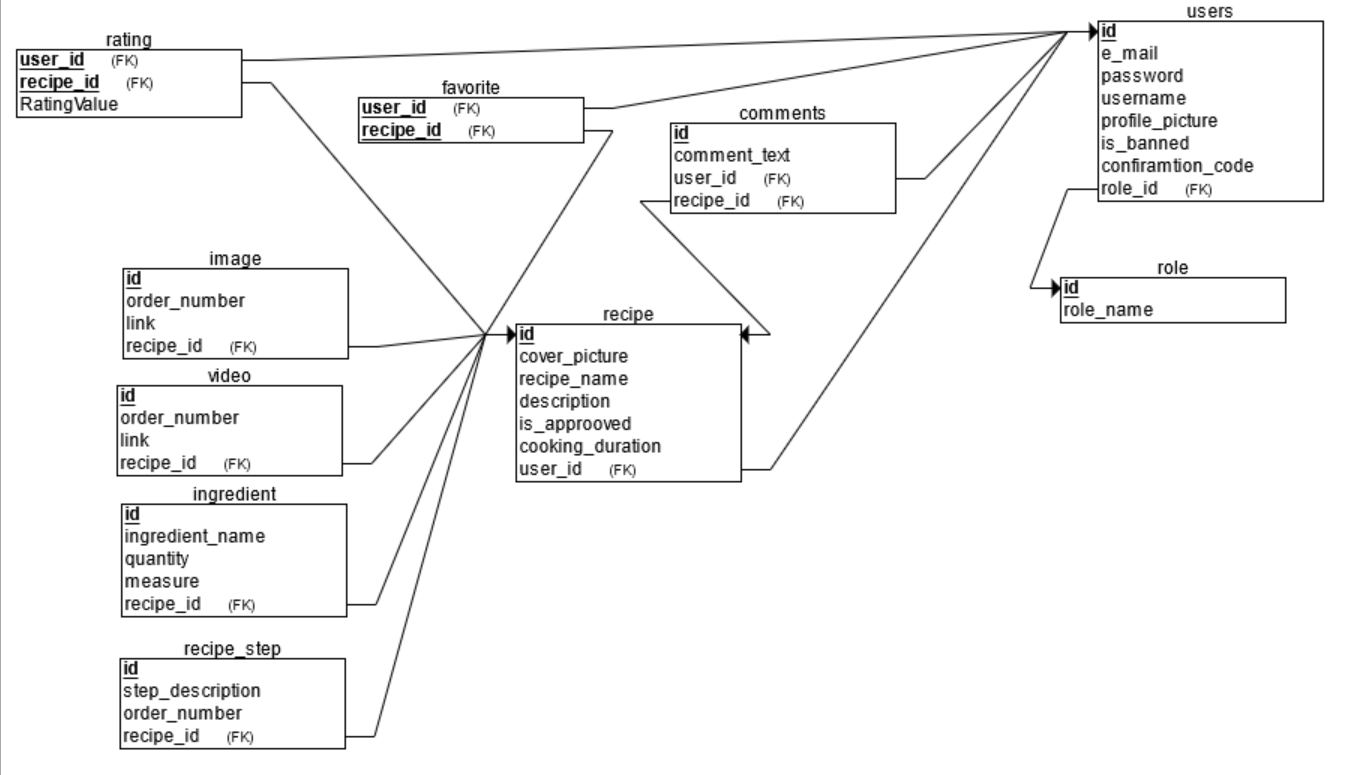
\includegraphics[width=\textwidth]{RelationalSchema.png}
      \caption{Relacijska shema}
      \label{fig:Relacijska shema}
\end{figure}

\begin{multicols}{2}
      \lstinputlisting[language=SQL,basicstyle=\scriptsize,caption={SQL kod},captionpos=b]{./code/database.sql}
      \label{lst:SQL kod}
\end{multicols}

\chapter{Poslužiteljska strana}
Poslužiteljska strana je pisana u programskom jeziku Java verzije 11, pritom koristeći
SpringBoot radni okvir. Kao arhitekturni stil korišten je GraphQL koji je alternativa REST-u.
Projekt je modeliran kao maven projekt, a za upravljanje njime je korišten Git alat. Za upogonjavanje
se također koristio \textit{AWS} i njihov \textit{ElasticBeanstalk} servis. U svrhe razvoja korišteno je okruženje VSCode.

\section{GraphQL}

\subsection{Povijest}
Jedan od većih problema dizajniranja web poslužitelja pa tako i samih web aplikacije u REST
arhitekturnom stilu je problem prekomjernog dohvata podataka odnosno nedovoljnog dohvata podataka
\textit{(eng. overfetching and underfetching)}. Ako bi se taj problem pokušao riješiti sa
stvaranjem više krajnjih točaka \textit{(eng. endpoint)}, a uz to i više prijenosnih objekata takozvanih \textit{DTO-ova (Data Transfer Object)},
došlo bi do nagomilavanja izvornog koda. Tako je tvrtka Facebook došla
do ideje GraphQL-a. Naime razvojni programeri su tada radili s velikim brojem podataka koji su
bili međusobno ugnježđenji i povezani na razne načine i da bi aplikacija radila dovoljno brzo
i efikasno bilo je nužno dohvatiti samo one podatke koji se uistinu i koriste, a da se pritom dohvaćaju sa
što manjeg broja krajnjih točaka.

\subsection{Definicija}
GraphQL je upitni jezik specifično dizajniran za korisničku stranu aplikacije da bi mogla
od puslužiteljske strane zatražiti i dobiti samo one podatke koji su potrebni. Također
dopušta i definiranje formata i oblika podataka koji će se zahtijevati od poslužiteljske strane, a
da se ujedno upiti šalju na samo jednu krajnju točku. U GraphQL-u postoje 2 vrste upita:
upiti i mutacije \textit{(eng. query and mutation)}, razlika je u tome što upiti služe za dohvaćanje podataka,
a mutacije za mijenjanje podataka.

\subsection{Implementacija}
Unatoč tome što GraphQL nudi puno izmjena i lakši pristup podacima u usporedi sa REST-om, implementacija
nije otežana. U okviru ovoga rada u \textit{pom.xml} datoteku u kojoj se dodaju ovisnosti \textit{(eng. dependencies)}
bilo je potrebno dodati 2 nove ovisnosti: graphql-spring-boot-starter, graphql-java-tools
i po potrebi treću ovisnost koja nudi mogućnost testiranja sučelja,
a ona je graphiql-spring-boot-starter (Slika \ref{fig:graphql}). Nakon toga ove ovisnosti zahtijevaju
izradu jedne datoteke u kojoj će pisati sve moguće vrste podataka koje se mogu tražiti, i sve
moguće upite koji se mogu primiti, a takva datoteka se najčešće imenuje schema.graphqls (slika \ref{fig:graphql} (b)).
U slučaju ovog rada podatci u shemi su bili ujedno i relacijski modeli iz baze podataka,
a upiti postoje razni i bili su dodavani jedan po jedan ovisno o potrebi aplikacije (Slika \ref{fig:graphql}).
Iz priložene slike vidimo da postoji velik broj mutacija i upita, ali to i dalje ne mijenja činjenicu da postoji
samo jedna krajnja točka koja je u ovom slučaju \textit{/graphql}, također je priložen primjer jednog tipa podatka: Recipe
i iz njegovog opisa je moguće primjetiti da je to upravo jedan od relacijskih modela iz baze podataka u koji su dodani
još neki dodatni parametri. Treba samo zapamtiti da se imena i tipovi polja iz Javine klase i tipa podatka iz
graphql sheme moraju podudarati jer se koristi refleksija za dohvat tih polja.
\begin{figure}[h]
      \centering
      \subfloat[\centering GraphQL ovisnosti]{{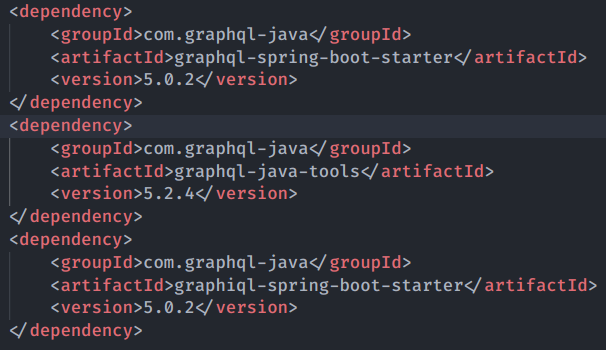
\includegraphics[width=.486\textwidth]{graphql_dependencies.png} }}
      \subfloat[\centering Primjer GraphQL sheme]{{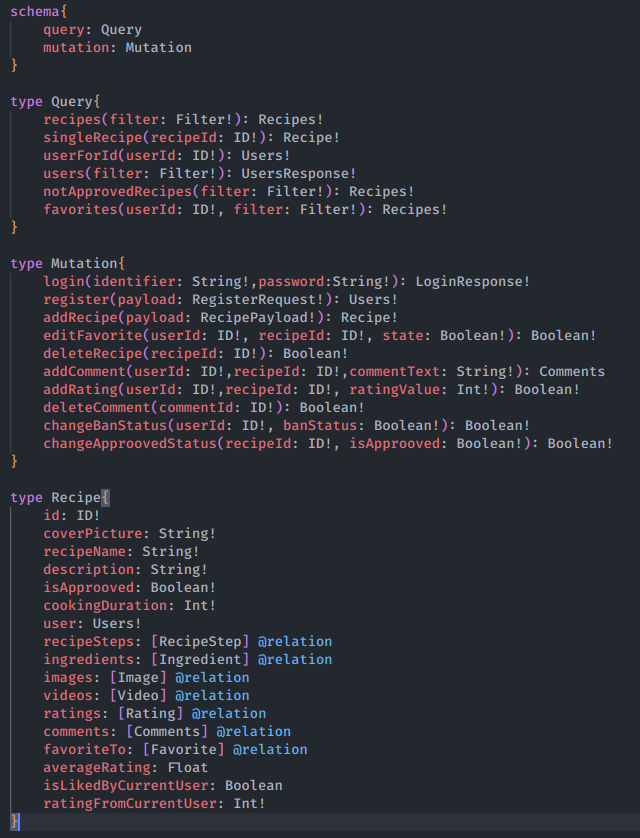
\includegraphics[width=.45\textwidth]{graphql_schema.png} }}
      \caption{GraphQL postavke}
      \label{fig:graphql}
\end{figure}
\\
Nakon dodavanja sheme i ovisnosti potrebno je dodati takozvane \textit{Resolvere}. U ovome projektu postoje 3 vrste resolvera:
QueryResolver, MutationResolver i obični Resolver, oni su u prethodno navedenim ovisnostima definirani kao sučelja:
GraphQLQueryResolver, GraphQLMutationResolver, GraphQLResolver. Prvi služi za prihvaćanje upita, drugi služi za prihvaćanje
mutacija, a treći služi za rješavanje problema spomenutih dodatnih parametara koji su umetnuti u GraphQL shemu,
na način da se definira način dohvata tih podataka. Također se može implementirati sučelje GraphQLErrorHandler koji
će presretati greške s poslužiteljske strane i vraćati odgovarajuću poruku korisničkoj strani, jer naime GraphQL
ima jednu manu, a ta mana je da se na korisničku stranu uvijek vraća HTTP status kod 200 OK, pa se rukovanje greškama
obavlja na drukčiji način. Taj način je da se u odgovor u slučaju greške doda parametar \textit{errors} koji će sadržavati
sve greške koje su se dogodile (slika \ref{fig:Handled error}).
Ako se ne implementira sučelje GraphQLErrorHandler poslužitelj će uvijek vraćati predefiniranu pogrešku (slika \ref{fig:Default error}). \\
\begin{figure}[h]
      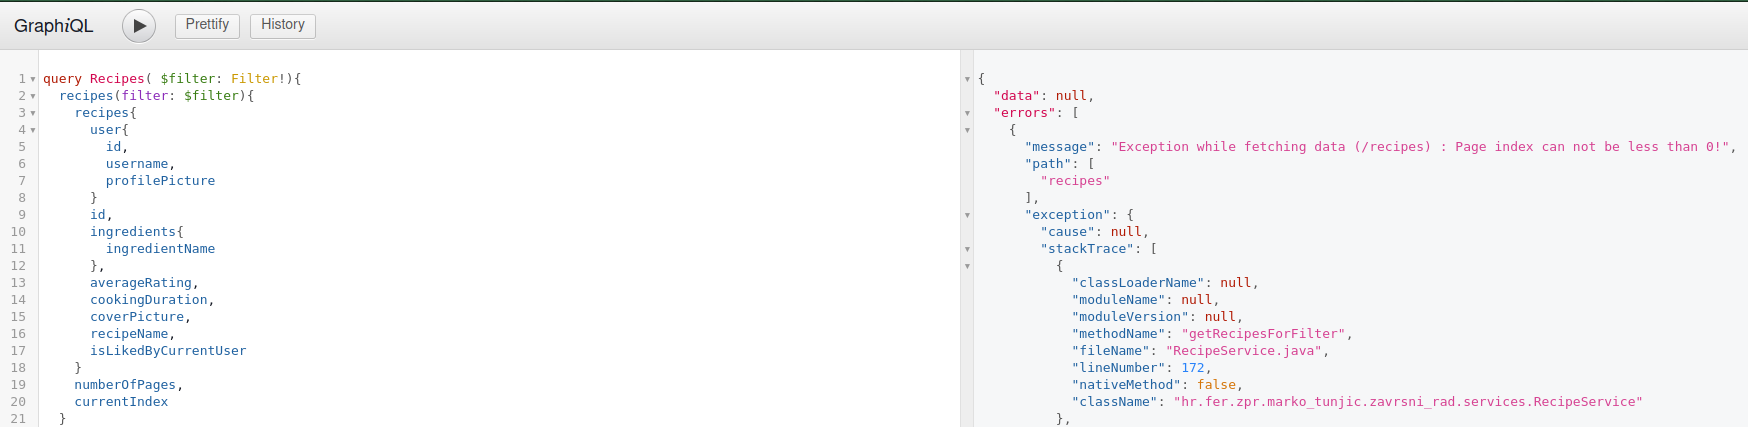
\includegraphics[width=\textwidth]{graphql_handled_error.png}
      \caption{Primjer greške ako postoji GraphQLErrorHandler}
      \label{fig:Handled error}
\end{figure}
\begin{figure}[h]
      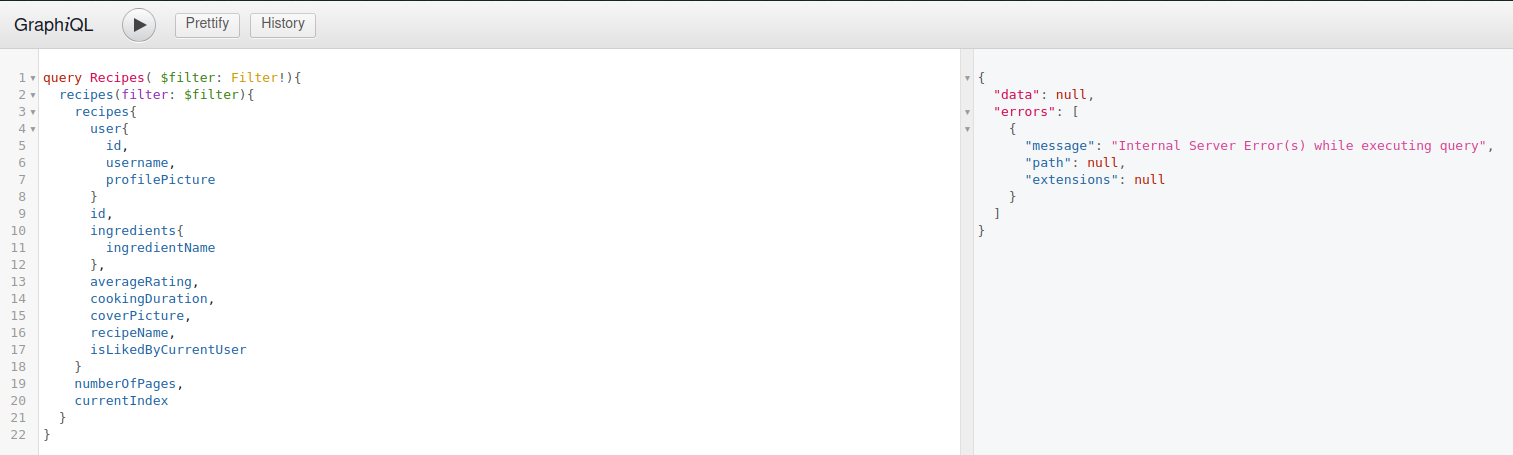
\includegraphics[width=\textwidth]{graphql_default_error.png}
      \caption{Primjer predefenirane pogreške}
      \label{fig:Default error}
\end{figure}
\\
Za kraj nakon implementacije svih navedenih sučelja (slika \ref{fig:GraphQL implementation}) sada se
uspješno može izvršiti prvi upit koji je demonstriran kroz sučelje \textit{GraphiQL} koji
prikazuje strukturu upita i odgovora (slika \ref{fig:GraphQL query}).
\begin{figure}[h]
      \centering
      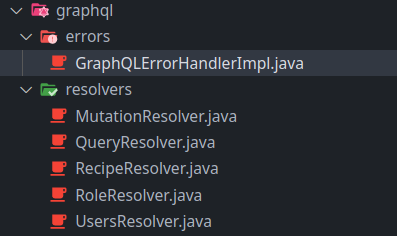
\includegraphics[width=.5\textwidth]{graphql_implementation_classes.png}
      \caption{Izgled graphql implementacije}
      \label{fig:GraphQL implementation}
\end{figure}
\begin{figure}[h]
      \centering
      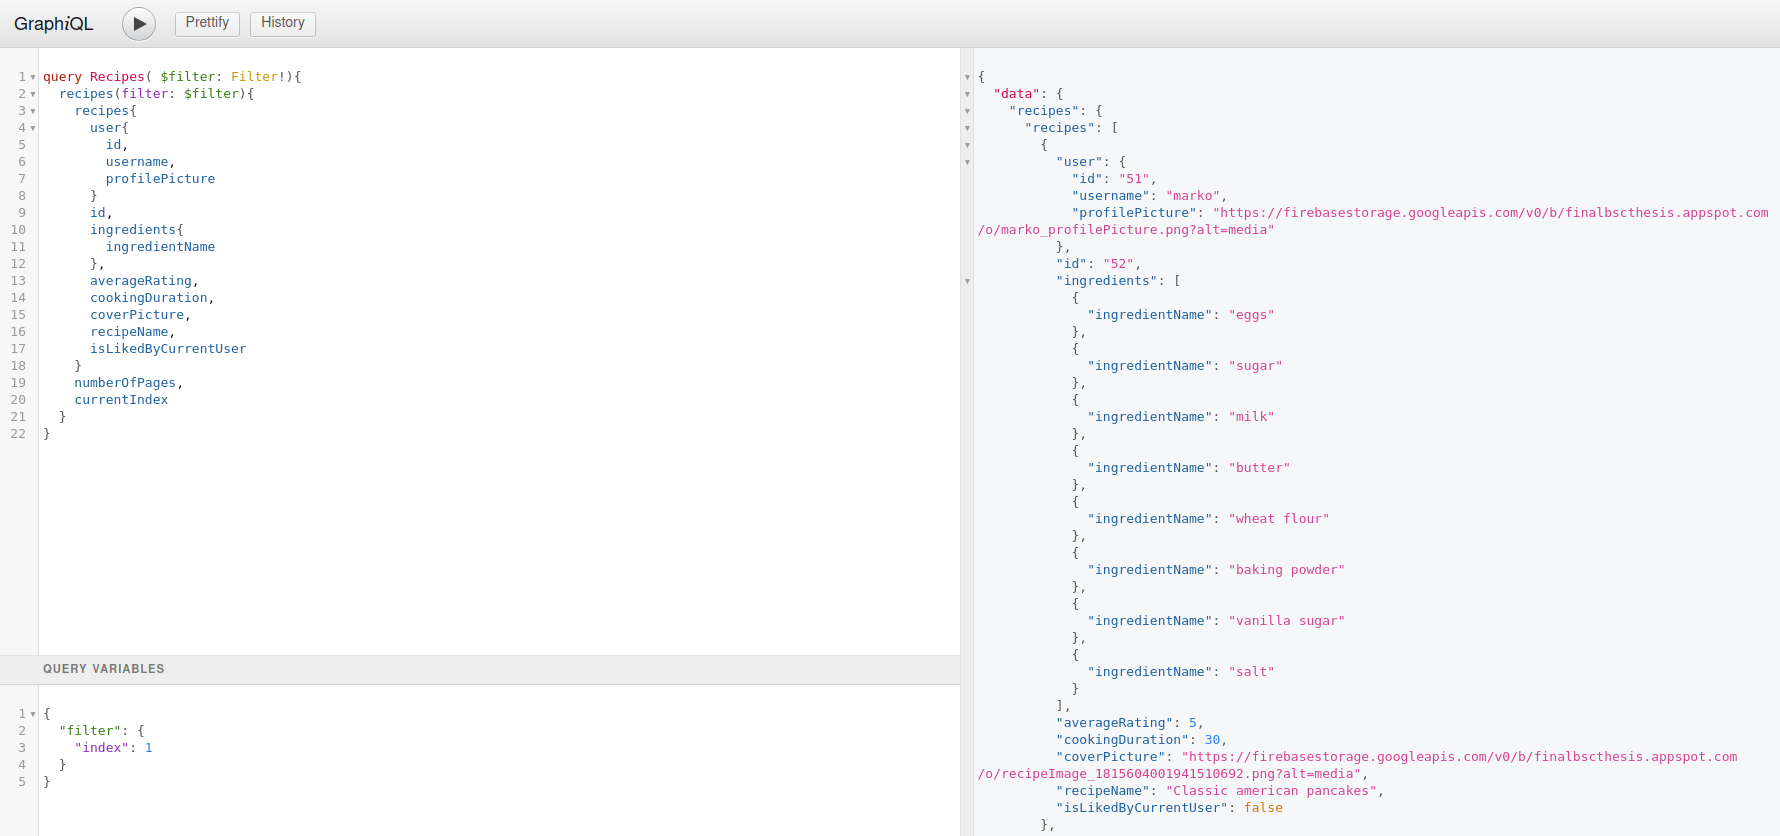
\includegraphics[width=\textwidth]{graphql_query.png}
      \caption{Primjer ispravnog upita}
      \label{fig:GraphQL query}
\end{figure}


\section{Autentifikacija i autorizacija}

\subsection{JWT}
U području autentifikacije i autorizacije se vidi jedna velika razlika između mobilne aplikacije i aplikacije koja
se pokreće na web pregledniku, a to je odsutnost sesije. Zato se mobilne aplikacije koriste drugim mehanizmom, a
to su tokeni. U ovoj aplikaciji se koriste tokeni pod imenom \textit{JWT (JSON Web Token)}, takvi tokeni koriste
kriptografske algoritme (kao na primjer HMACSHA256) da bi se podatci na siguran način mogli prenositi između dvije strane.
Pa će se u takvom tokenu nalaziti korisničko ime, istek tokena i slični podatci koji će omogućiti
autentifikaciju i autorizaciju korisnika aplikacije.

\subsection{Autentifikacija}
Da bi se ovo ostvarilo prvo je bilo potrebno dodati ovisnost prema \linebreak
SpringSecurity-u (slika \ref{fig:Security dependency}) i prema jjwt. Nakon toga da bi aplikacija mogla doći do podataka trebalo je implementirati dva sučelja:
\textit{UserDetails} i \textit{UserDetailsService}. Prvo sučelje služi za omotavanje osnovnih podataka o korisniku,
kao na primjer korisničko ime, lozinka, je li korisnik suspendiran, je li korisnik potvrdio svoj identitet,
koje su korisnikove uloge (administrator ili korisnik) i slično,
a drugo sučelje služi za dohvat tih podataka na osnovu korisničkog imena. U ovoj aplikaciji sučelje UserDetails omotava
podatke iz baze podataka, a drugo sučelje dohvaća podatke iz baze i sprema ih u prvo sučelje.
\begin{figure}[h]
      \centering
      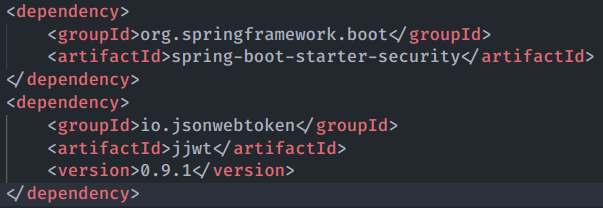
\includegraphics[width=.5\textwidth]{security_dependency.png}
      \caption{Ovisnost za autentifikaciju i autorizaciju}
      \label{fig:Security dependency}
\end{figure}
\\
Nadalje da bi se ti podatci mogli dohvatiti u bilo kojem trenutku potrebno ih je spremiti negdje u nekom trenutku.
Zato je bilo potrebno napraviti jedan \textit{Filter}. \textit{Filteri} su posebni objekti u web aplikaciji koji presreću bilo koji
zahtjev koji stigne na poslužitelj, obrade taj zahtjev i onda ga proslijede dalje prema web aplikaciji.
Filter za autentifikaciju će provjeriti postoji li HTTP zaglavlje pod imenom: \textit{Authorization} i ako
postoji pretpostaviti će da se unutra nalazi token kojeg će pokušati isparsirati i iz njega dohvatiti korisničko ime.
Na osnovu tog korisničkog imena i uz pomoć sučelja \textit{UserDetailsService} vrlo jednostavno se dohvati sučelje \textit{UserDetails}.
Na kraju će filter spremiti bitne podatke u takozvani \textit{SecurityContextHolder} koji će pružiti mogućnost dohvata trenutnog
korisnika u bilo kojem trenutku.
\\\\
Jedan od mogućih scenarija je da će podatci poslani u tokenu biti ili nevažeći ili isteknuti zato je potrebno napraviti
takozvani \textit{EntryPoint} koji će u slučaju pogrešne autorizacije korisniku vratiti odgovarajuću poruku. Taj EntryPoint
se naziva \textit{AuthenticationEntryPoint} koji će preko HTTP odgovora poslati pogrešku u svojoj metodi commence. Struktura
svih implementiranih sučelja u projektu prikazana je na slici \ref{fig:Security}

\begin{figure}[h]
      \centering
      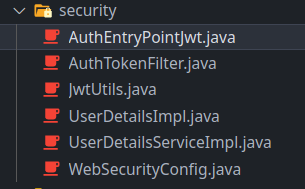
\includegraphics[width=.5\textwidth]{security_implementation.png}
      \caption{Struktura sigurnosnog dijela}
      \label{fig:Security}
\end{figure}

\subsection{Autorizacija}
Na kraju je potrebno definirati autorizaciju i spojiti s autentifikacijom, a to se obavlja kroz takozvani WebSecurityConfig.
U kojem je definirano koji će se EntryPoint koristiti u slučaju pogreške, koji algoritam se koristi za šifriranje lozinki,
kada se poziva filter za autentifikaciju i kada se obavlja autorizacija. U ovoj aplikaciji se koristi prethodno
definirani \textit{EntryPoint}, za šifriranje lozinke se koristi \textit{BCrypt} algoritam, filter se poziva prije svakog zahtjeva, a
autorizacija je omogućena da se definira za svaku metodu zasebno uz pomoć anotacije \textit{@PreAuthorize} (slika \ref{fig:WebSecurityConfig}).
Ta anotacija se koristi na način da se u tijelo anotacije stave sve uloge koje smiju pristupati anotiranoj metodi (slika \ref{fig:PreAuthorize}).
One se najčešće stavljaju ili u \textit{QueryResolver-u} ili u \textit{MutationResolver-u} i tako će se ograničiti pristup
neautorizirani korisnicima.
\begin{figure}[h]
      \centering
      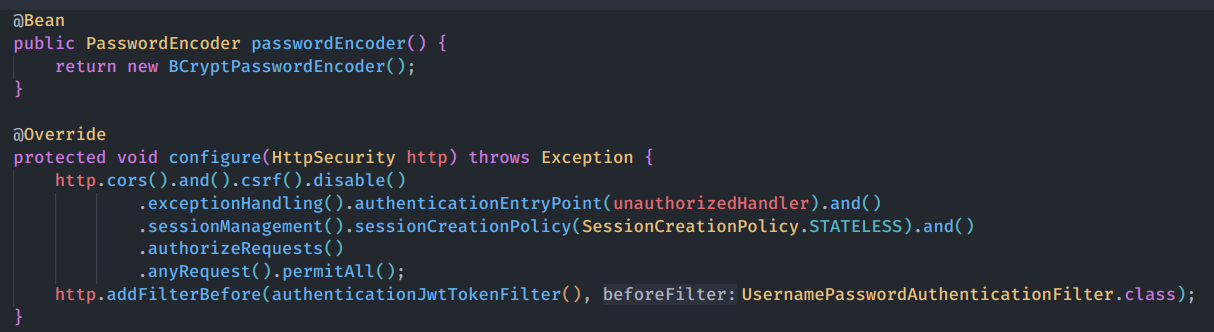
\includegraphics[width=\textwidth]{WebSecurityConfig.png}
      \caption{Izgled sigurnosne konfiguracije}
      \label{fig:WebSecurityConfig}
\end{figure}
\begin{figure}[h]
      \centering
      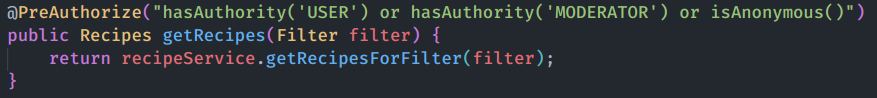
\includegraphics[width=\textwidth]{PreAuthorize.png}
      \caption{Izgled metode s anotacijom @PreAuthorize}
      \label{fig:PreAuthorize}
\end{figure}

\section{Pristup podacima}
Za pristup podacima se koriste dva sloja prvi sloj je sloj za perzistenciju, a drugi sloj je sloj usluge. Sloj za perzistenciju
modeliran je uz pomoć takozvanog \textit{ORM-a (Object Realtional Mapper)} čija je zadaća preslikavanje relacija u Javine objekte.
Postoji više vrsta različitih ORM-ova, a u ovome projektu se koristi \textit{Hibernate}. Za sve to je bilo potrebno dodati ovisnost prema odgovarajućim
\textit{JPA} i \textit{JDBC} maven ovisnostima (slika \ref{fig:Data dependencies} (a)).
\begin{figure}[h]
      \centering
      \subfloat[\centering Ovisnosti]{{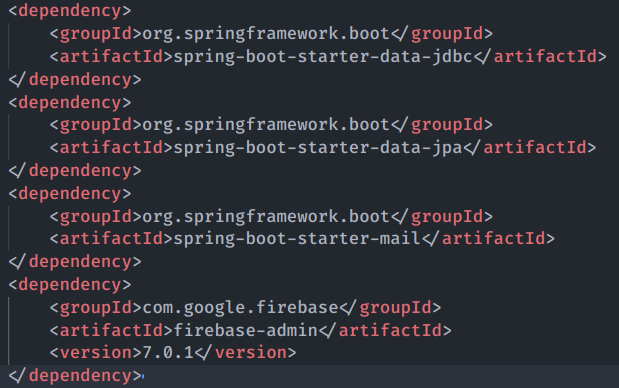
\includegraphics[width=.486\textwidth]{data_dependencies.png} }}
      \subfloat[\centering Sve usluge]{{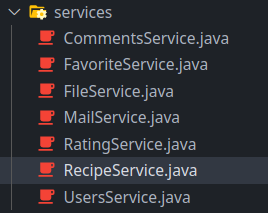
\includegraphics[width=.45\textwidth]{services.png} }}
      \caption{Ovisnosti za pristup podacima i sloj usluge}
      \label{fig:Data dependencies}
\end{figure}

\subsection{Sloj za perzistenciju}
U programskom jeziku java, hibernate se koristi kroz JPA (Java Persistence API) programsko sučelje.
JPA zahtijeva da se način preslikavanja iz relacije u objekt definira ili anotacijama
ili u posebnoj konfiguracijskoj datoteci, u ovome projektu je to učinjeno preko anotacija, a sve takve klase prikazane su na
slici \ref{fig:JPA} (a). Anotacije i način anotiranja koji se mora poštivati prikazan je na slici \ref{fig:JPA} (b). Može se primjetititi
da u modelima ovoga projekta nisu anotirane sve veze koje su određene samom bazom podataka
jer je to riješeno uz pomoć \textit{Resolvera} iz \textit{GraphQL-a}. Nakon kreiranja svih modela potrebno je napraviti sučelja koja nasljeđuju sučelje
\textit{JPARepository} preko kojeg se pristupa samim podacima, a u tom sučelju su definirane metode kao na primjer metoda
za dohvaćanje svih relacija, metoda za dohvaćanje relacija po identifikacijskom atributu, ili nekom drugom atributu
i slične metode.
\begin{figure}[h]
      \centering
      \subfloat[\centering Svi anotirani modeli]{{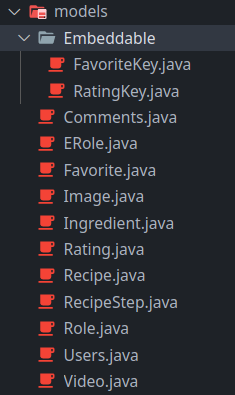
\includegraphics[width=.486\textwidth]{models.png} }}
      \subfloat[\centering Primjer anotiranja klase]{{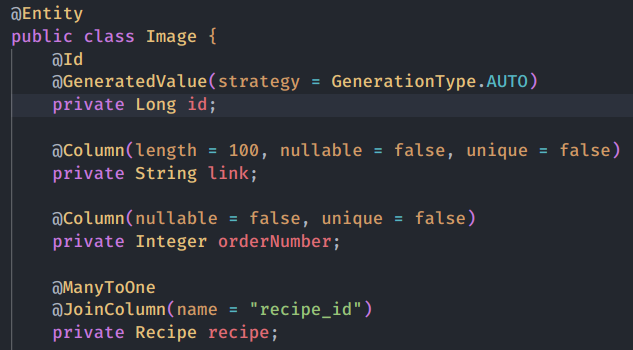
\includegraphics[width=.45\textwidth]{jpa_annotations.png} }}
      \caption{JPA konfiguracija}
      \label{fig:JPA}
\end{figure}
\\\\
Također iz slike \ref{fig:JPA} (b) može se primjetiti da se slika u bazu sprema kao hiperveza na samo sliku, a to je moguće jer se za
spremanje slika koristi \textit{firebase}. Za pristup firebase-u je bilo potrebno dodati ovisnost (slika \ref{fig:Data dependencies}) i jednu datoteku u kojoj su zapisani
podaci za pristup bazi koja iz sigurnosnih razloga nije priložena. Nakon je toga je vrlo lako uz pomoć metode \textit{create} primljenu
sliku "dignuti" na \textit{firebase oblak}.

\subsection{Sloj usluge}
Jedno od SOLID načela programiranja (\textit{"Single responsibility"}) nalaže da jedna klasa ima samo jednu odgovornost
zato je sloj za perzistenciju od \textit{resolver-a} odvojen slojem usluge. U sloju usluge se nalazi sva logika
potrebna za pristup i obradi podatka da bi se razdvojila odgovornost obrade podataka od odgovornosti obrade zahtjeva.
\\\\
Također osim same obrade podataka u sloju usluge se nalazi i klasa koja služi za slanje elktroničke pošte.
Ta usluga se koristi za slanje poruke za potvrdu identiteta i za slanje liste za kupnju
koja se šalje ako neki korisnik doda recept u svoje favorite. Tijelo poruke se gradi
kao HTML dokument, a šalje se uz pomoć \textit{Java Mail API-a} za koji je bilo potrebno dodati ovisnost
prikazanu na slici \ref{fig:Data dependencies}. I konačno sve usluge su prikazane na slici \ref{fig:Data dependencies} (b).

\section{Upogonjavanje}
Upogonjavanje se obavlja uz pomoć github actions gdje je definiran takozvani \textit{CI/CD pipeline}
(slika \ref{fig:Backend cicd}) uz pomoć kojeg se izvorni kod prevodi u .jar arhivu i podiže na \textit{AWS ElasticBeanstalk} servis.
Jedini problem je bio što nakon upogonjavanja poslužitelj može primati relativno male zahtjeve
, a za ovu aplikaciju su potrebni poprilično veliki zahtjevi jer se šalju i fotografije i videozapisi
zato se uz .jar arhivu mora dodati i konfiguracijska datoteka za \textit{ngnix} poslužitelj koja će povećati
pretpostavljenu maksimalnu veličinu zahtjeva. To je postignuto uz pomoć maven-ovog \textit{"antrun plugin-a"}
(slika \ref{fig:antrun}) koji će .jar arhivu i konfiguracijsku datoteku spremiti u .zip arhivu i proslijediti to dalje.
\begin{figure}[h]
      \centering
      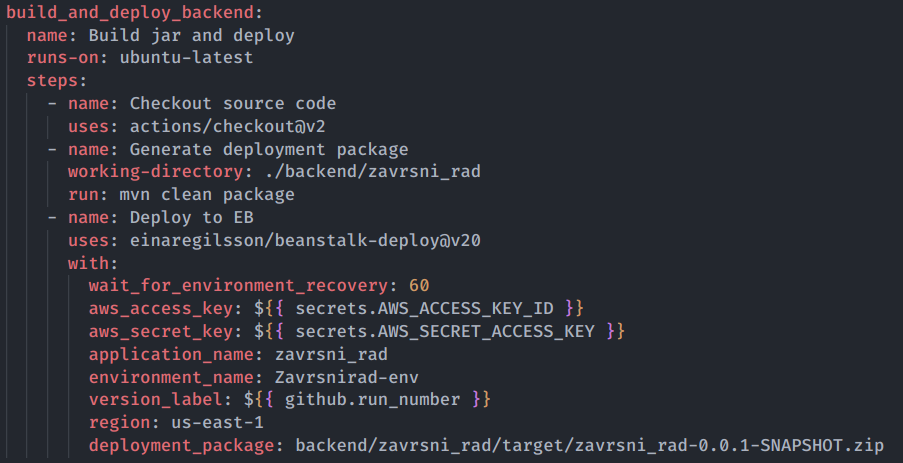
\includegraphics[width=.5\textwidth]{backend_cicd.png}
      \caption{Github actions zadatak za podizanje web poslužitelja}
      \label{fig:Backend cicd}
\end{figure}
\begin{figure}[h]
      \centering
      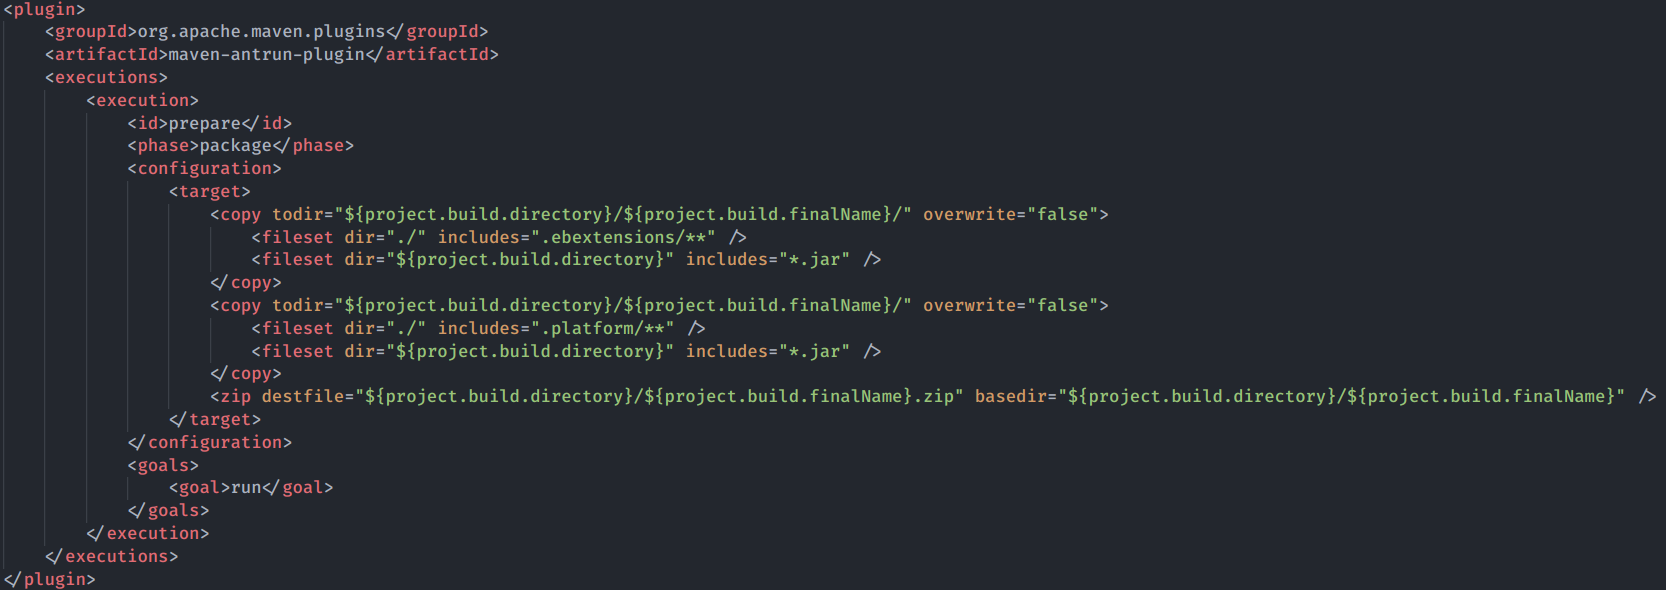
\includegraphics[width=\textwidth]{antrun.png}
      \caption{Plugin za stvaranje zip arhive za upogonjavanje}
      \label{fig:antrun}
\end{figure}

\chapter{Korisnička strana}
Korisnička strana je pisana u programskom jeziku dart, pritom koristeći
Flutter radni okvir. Struktura projekta je napravljena potpuno slobodno (slika \ref{fig:Frontend}(a)).
Za komunikaciju s poslužiteljskom stranom korišten je paket flutter-graphql.
Za upogonjavanje aplikacije korištena je github-ova mogućnost
stvaranja izdanja, a sam proces upogonjavanja je obavljeno uz pomoć \textit{github actions} (slika \ref{fig:Frontend})(b).
U svrhe razvoja korišteno je okruženje VSCode.
\begin{figure}[h]
      \centering
      \subfloat[\centering Izgled strukture projekta]{{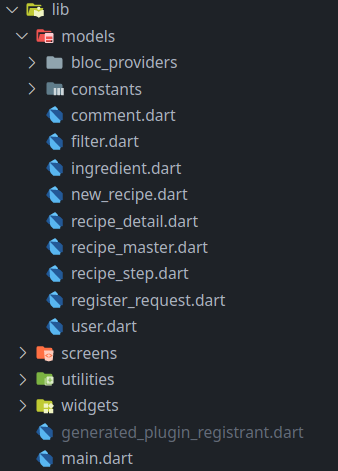
\includegraphics[width=.486\textwidth]{frontend_structure.png} }}
      \subfloat[\centering GitHub actions za upogonjavanje aplikacije]{{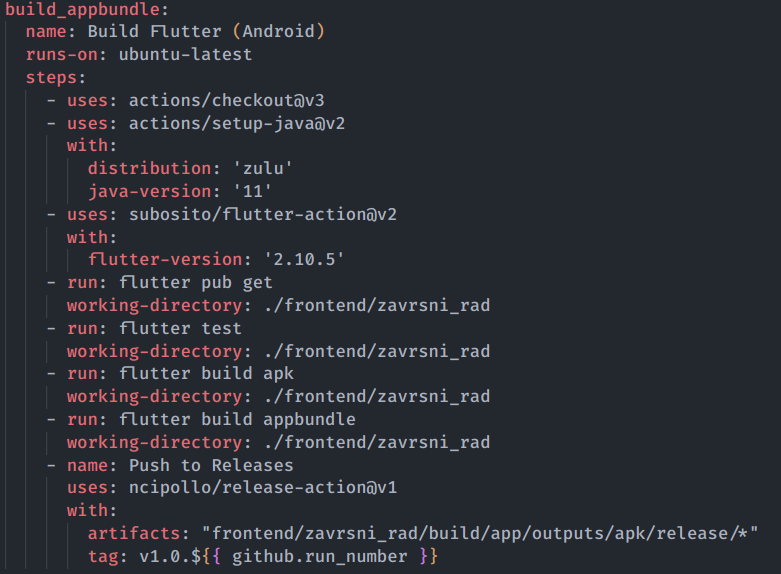
\includegraphics[width=.45\textwidth]{frontend_cicd.png} }}
      \caption{Osnovne karakteristike korisničke strane}
      \label{fig:Frontend}
\end{figure}

\section{Flutter}
Flutter je google-ov javno dostupni (\textit{eng. Open Source}) projekt koji je namijenjen
za stvaranje lijepih i brzih mobilnih, web, računalnih ili ugrađenih aplikacija. Karakteristika
\textit{flutter-a } je da se aplikacija sa samo jednim programskim kodom može pokrenuti u
svim navedenim okruženjima. Također jedna od prednosti tog radnog okvira je da je vrlo lako napraviti
dinamične aplikacije jer se koristi upravljanje stanjem (eng. \textit{state managment}). Postoji više načina
kako pristupiti ovoj funkcionalnosti, a u ovome radu korištem je \textit{BLoC} pristup koji je ujedno
i google-ov preporučeni pristup.
\\\\
Također se sadržaj dinamički mijenja u ovisnosti o upitima na poslužiteljsku stranu i ta dinamičnost
se postiže uz pomoć \textit{widget-a} namijenjenih za slanje \textit{graphql} upita koji se zovu \textit{Query i Mutation}.
Navedeni \textit{widget-i} imaju jednu funkciju koja se poziva svaki put kada se promjeni stanje upita i
zove se \textit{builder}. Toj funkciju se kao ulazni parametar šalje rezultat i stanje izvođenja upita to jest mutacije,
i dužnost joj je vratiti \textit{widget} koji će se prikazati na ekranu.

\subsection{BLoC}
BLoC (Business Logic Components) je obrazac za upravljanjem stanjem aplikacije. Karakteristika ovog obrasca
je da međusobno razdvaja prikaz komponente, upravljanje njenim stanjem i logiku iza upravljanja stanjem.
Srž obrasca je načelo da bi sve u aplikaciji trebalo biti modelirano kao tok događaja, na način da jedna komponenta
na osnovu interakcije s okolinom kreira događaje i šalje ih u ulazni tok događaja, a svaka komponenta koja
ovisi o tom toku događaja će kroz izlazni tok događaja primiti te podatke i na osnovu njih ažurirati svoje stanje.
\begin{figure}[h]
      \centering
      \subfloat[\centering BLoCProvider i modeli događaja]{{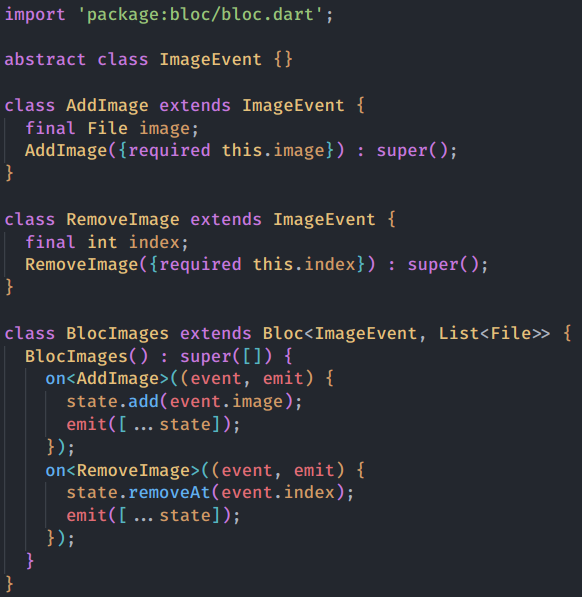
\includegraphics[width=.486\textwidth]{bloc_provider.png} }}
      \subfloat[\centering Primjer BLoCBuilder-a]{{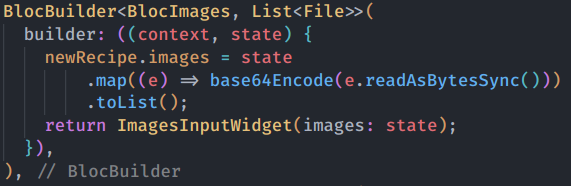
\includegraphics[width=.45\textwidth]{bloc_builder.png} }}
      \caption{Implementacija BLoC-a}
      \label{fig:BLoC}
\end{figure}
U implementaciji se to postiže uz pomoć 3 stvari: prvo klase koje predstavljaju događaje (u njima se mogu prenositi
potrebni podaci) (slika \ref{fig:BLoC} (a)), drugo \textit{BlocProvider} (slika \ref{fig:BLoC} (a))
i treće \textit{BlocBuilder} (slika \ref{fig:BLoC} (b)). \textit{BlocProvider} predstavlja dio \textit{BLoC-a}
koji se bavi presretanjem svakog ulaznog događaja, obrađivanjem i slanjem u izlazni tok, a \textit{BlocBuilder}
služi za izgradnju komponente na osnovu trenutnog događaja u izlaznom toku događaja.

\section{Ekrani}
U radnom okviru flutter ne postoji razlika između ekrana (eng \textit{screen}) i na primjer teksta jer je sve definirano
kao takozvani \textit{"widget"}, ali iz semantičkih razloga svaku skupinu \textit{widget-a} koja
se prikazuje u istome trenutku nazivamo ekran. Često se broj ekrana uzima kao stupanj
složenosti aplikacije. Tako ovaj rad ima 9 ekrana, ali oni nisu dostupni svim korisnicima nego
su podijeljeni po ulogama.

\subsection{Ekran dobrodošlice, prijave i registracije}
Ekran dobrodošlice (slika \ref{fig:WelcomeLogin} (a)) nema nekakvu posebnu namjenu osim estetske to jest da bi
korisniku ostavila dobar dojam. Također karakteristika ekrana dobrodošlice je
da se prikazuje samo jednom i to kada se aplikacija prvi puta pokreće na trenutnom
uređaju. To svojstvo se postiže podizanjem zastavice u memoriji uređaja uz pomoć
sučelja \textit{"SharedPreferences"}.
\begin{figure}[h]
      \centering
      \subfloat[\centering Ekran dobrodošlice]{{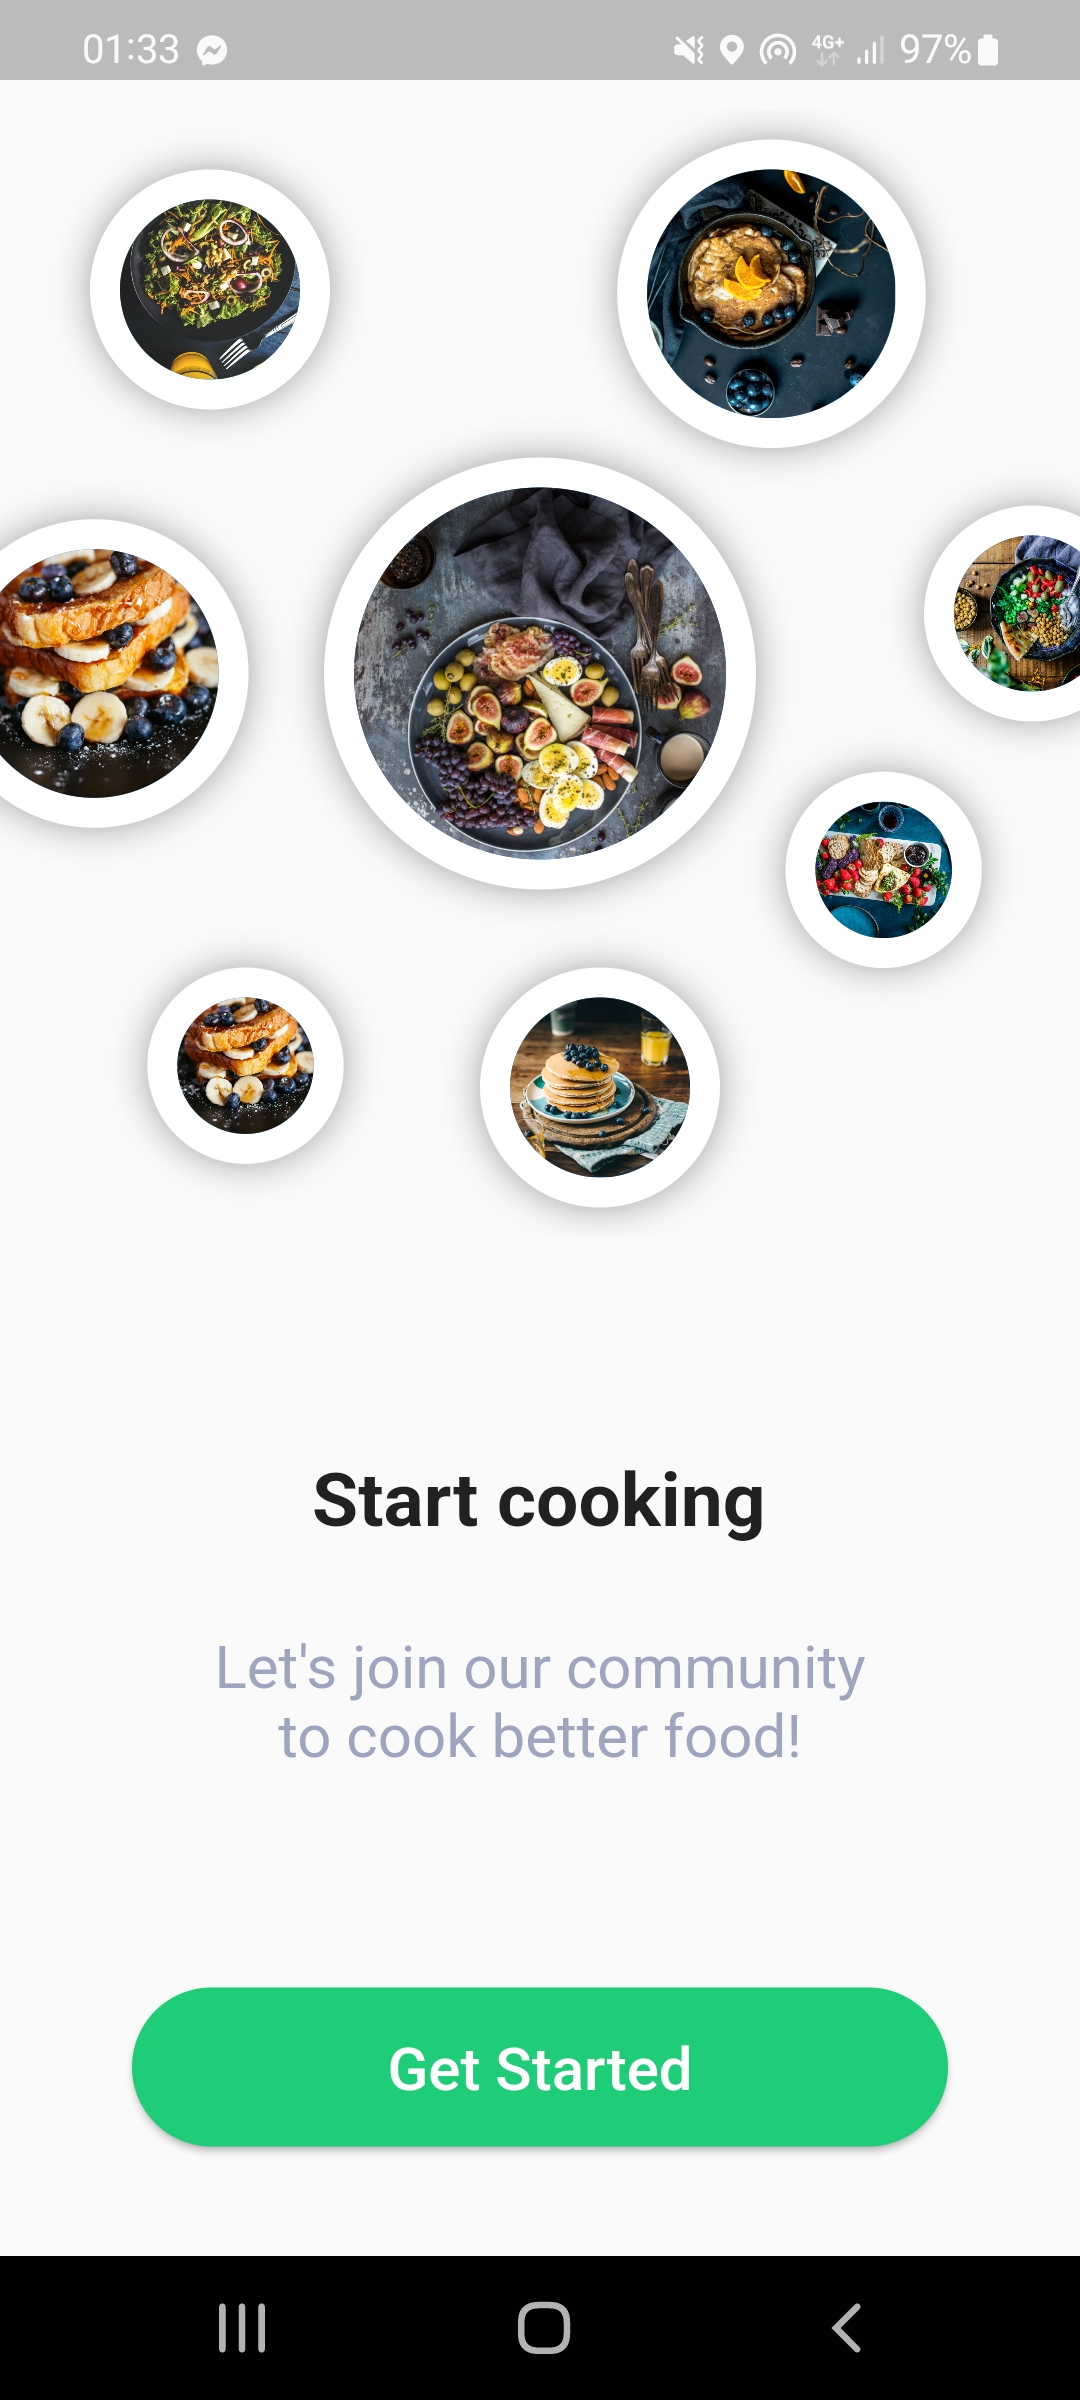
\includegraphics[width=.26\textwidth]{welcome_screen.jpg} }}
      \subfloat[\centering Ekran prijave]{{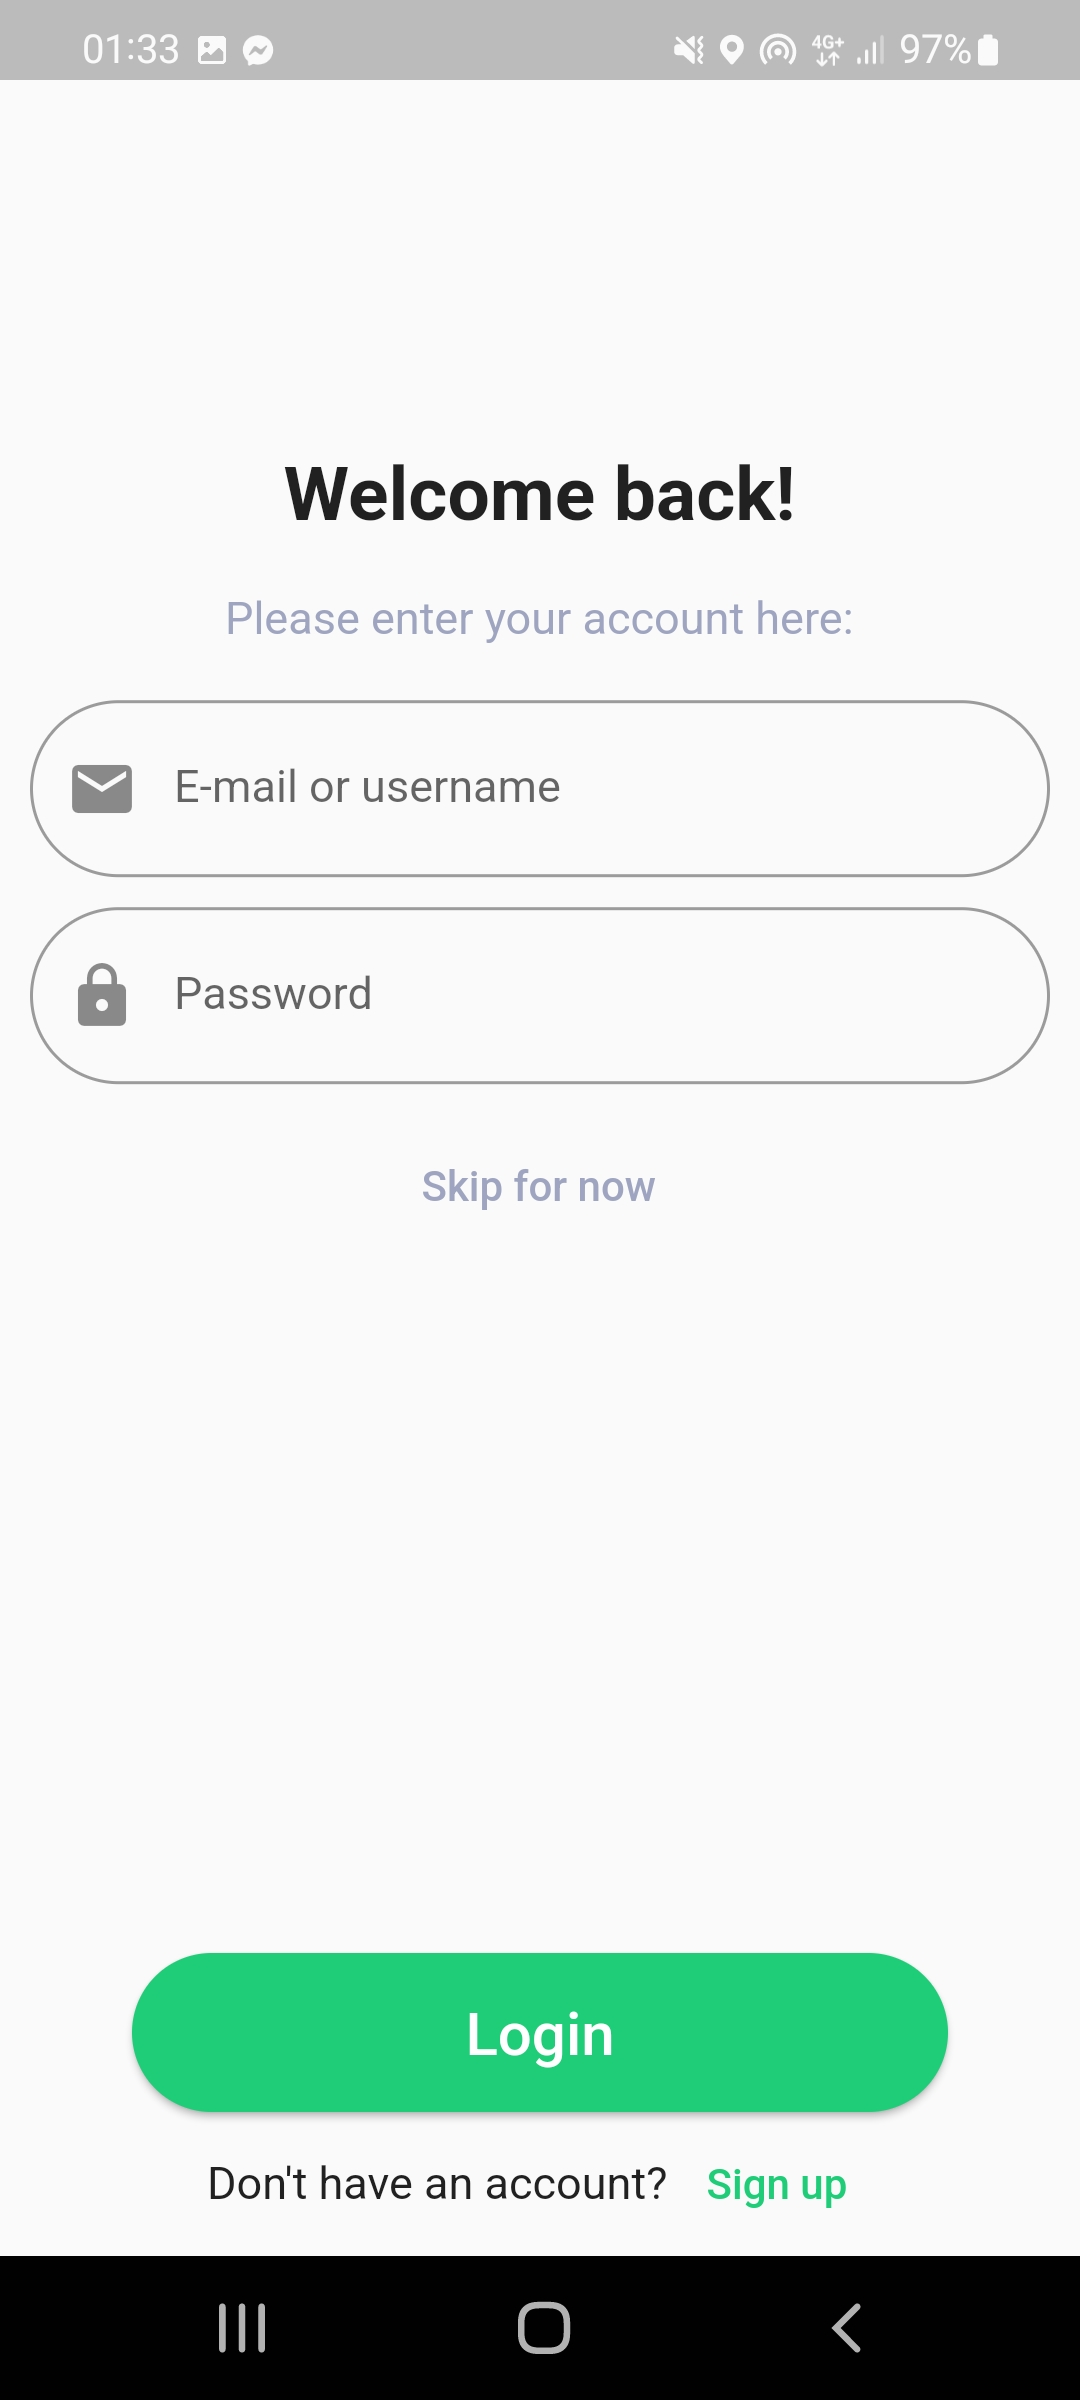
\includegraphics[width=.26\textwidth]{login_screen.jpg} }}
      \subfloat[\centering Ekran prijave u slučaju pogreške]{{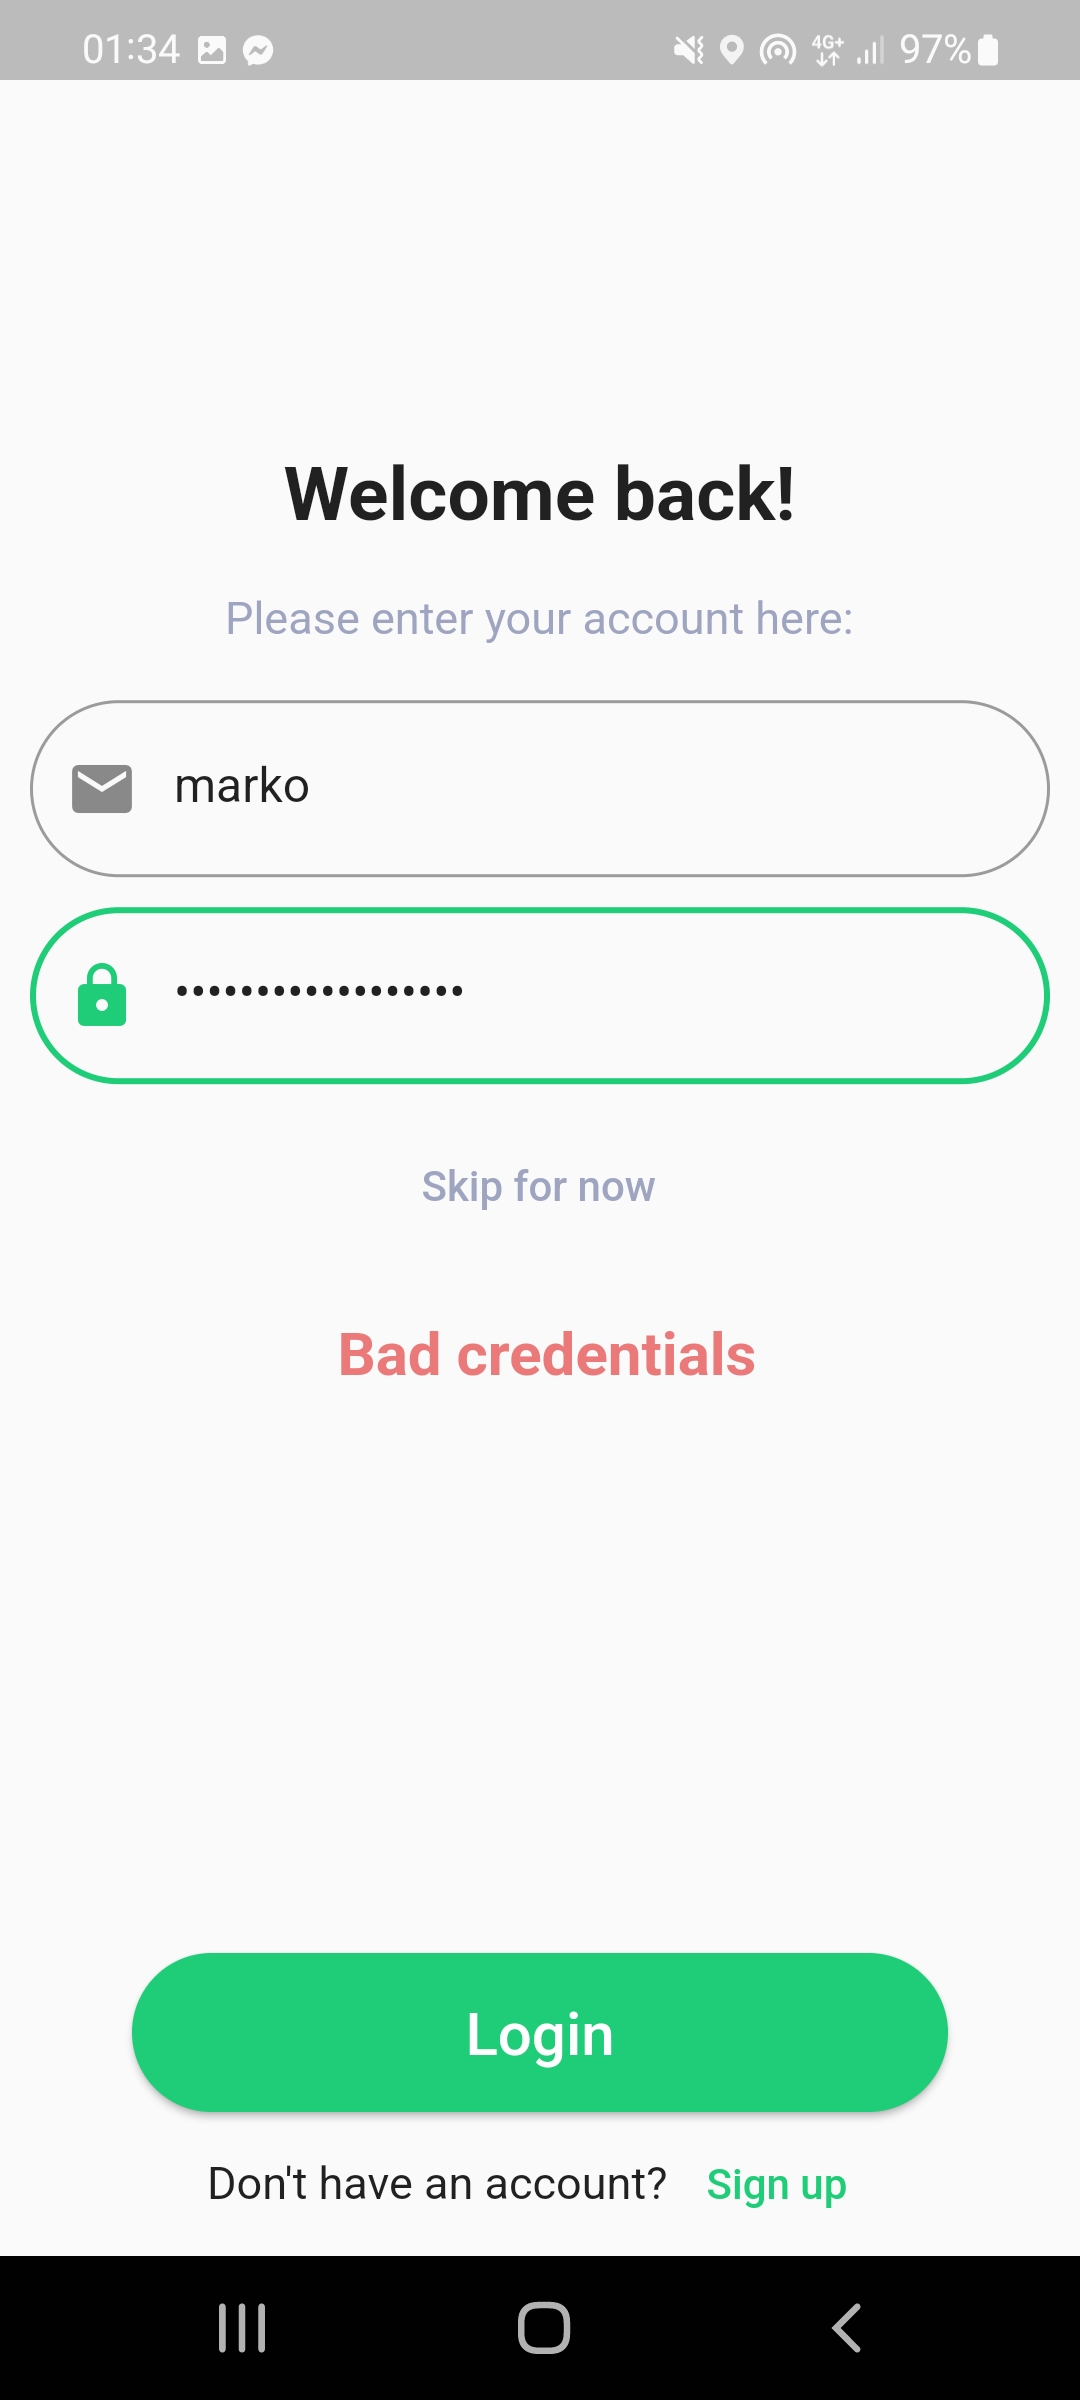
\includegraphics[width=.26\textwidth]{login_failed.jpg} }}
      \caption{Ekran dobrodošlice i prijave}
      \label{fig:WelcomeLogin}
\end{figure}
Ekran za prijavu sadrži 2 polja za unos i 3 gumba (slika \ref{fig:WelcomeLogin} (b)). Prvo polje je polje za unos
korisničkog imena ili e-pošte, drugo polje je polje za unos pripadajuće lozinke. Ako je uneseno
krivo korisničko ime ili lozinka prikazuje se odgovarajuća poruka (slika \ref{fig:WelcomeLogin} (c)). Nadalje
prvi gumb je gumb za preskakanje prijave i prelazak na stranicu sa svim receptima, drugi gumb je gumb
za potvrdu prijave, a treći gumb je gumb za prelazak na ekran za registraciju.
\\\\
Ekran za registraciju sadrži 5 polja za unos: unos računa elktroničke pošte, unos
korisničkog imena, unos lozinke, potvrda lozinke i odabir profilne slike koje je, za
razliku od ostalih polja opcionalno polje te 2 gumba (slika \ref{fig:Register} (a)). Karakteristika polja za lozinku je da ima posebne
validacijske kriterije, koji zahtijevaju da lozinka mora
sadržavati barem 8 znakova, jedno veliko slovo i jedan specijalni znak. Nakon uspješne registracije
prikaže se poruka da je registracija uspješno izvršena (slika \ref{fig:Register} (b)) i da je potrebno izvršiti potvrdu identiteta
putem e-mail račun-a koji je bio unesen.
\begin{figure}[h]
      \centering
      \subfloat[\centering Ekran neuspješne registracije]{{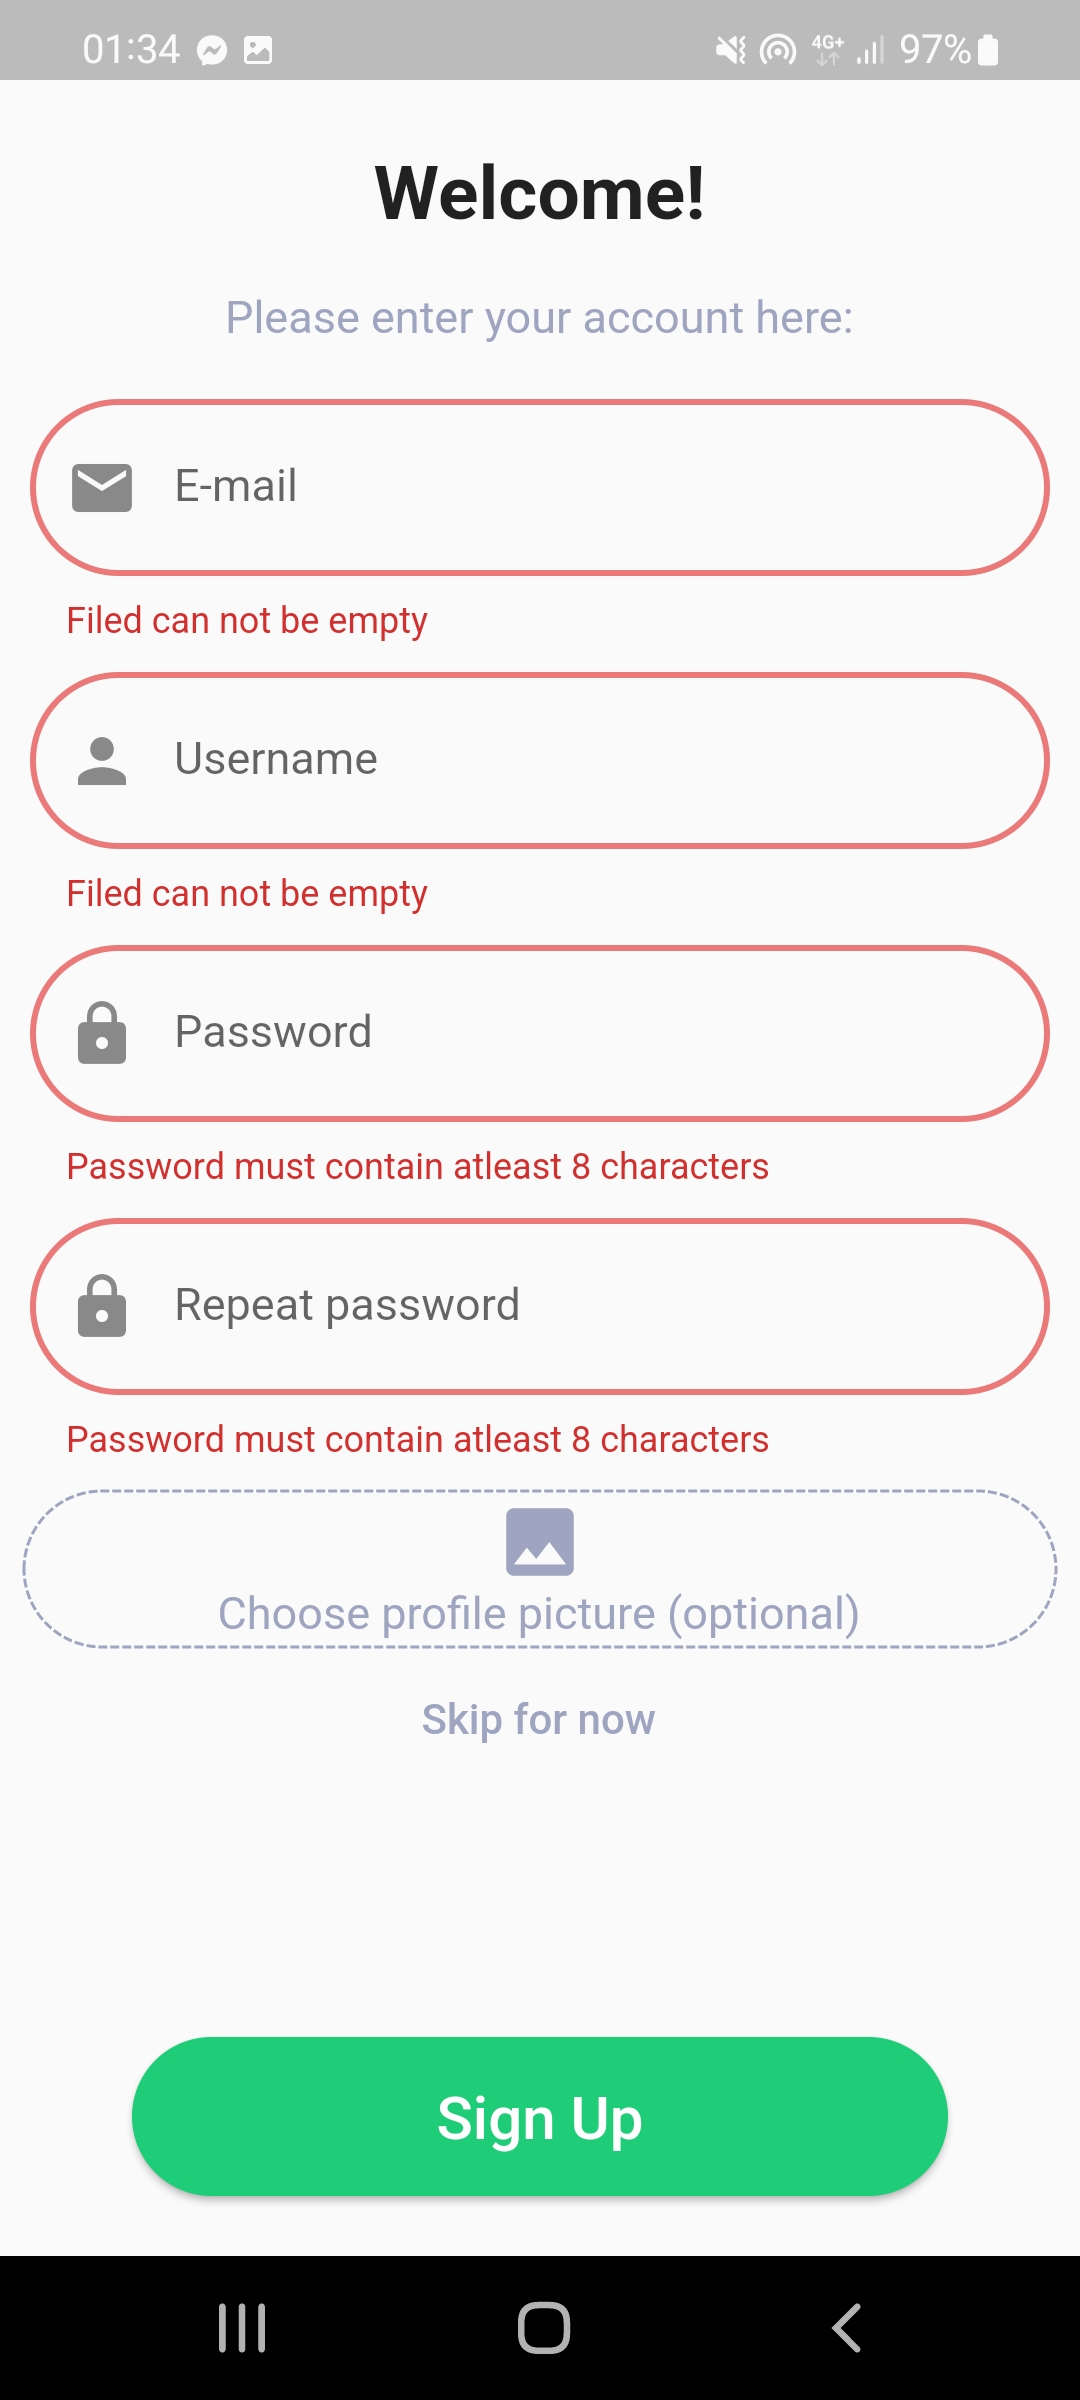
\includegraphics[width=.32\textwidth]{register_failed.jpg} }}
      \subfloat[\centering Ekran uspješne registracije]{{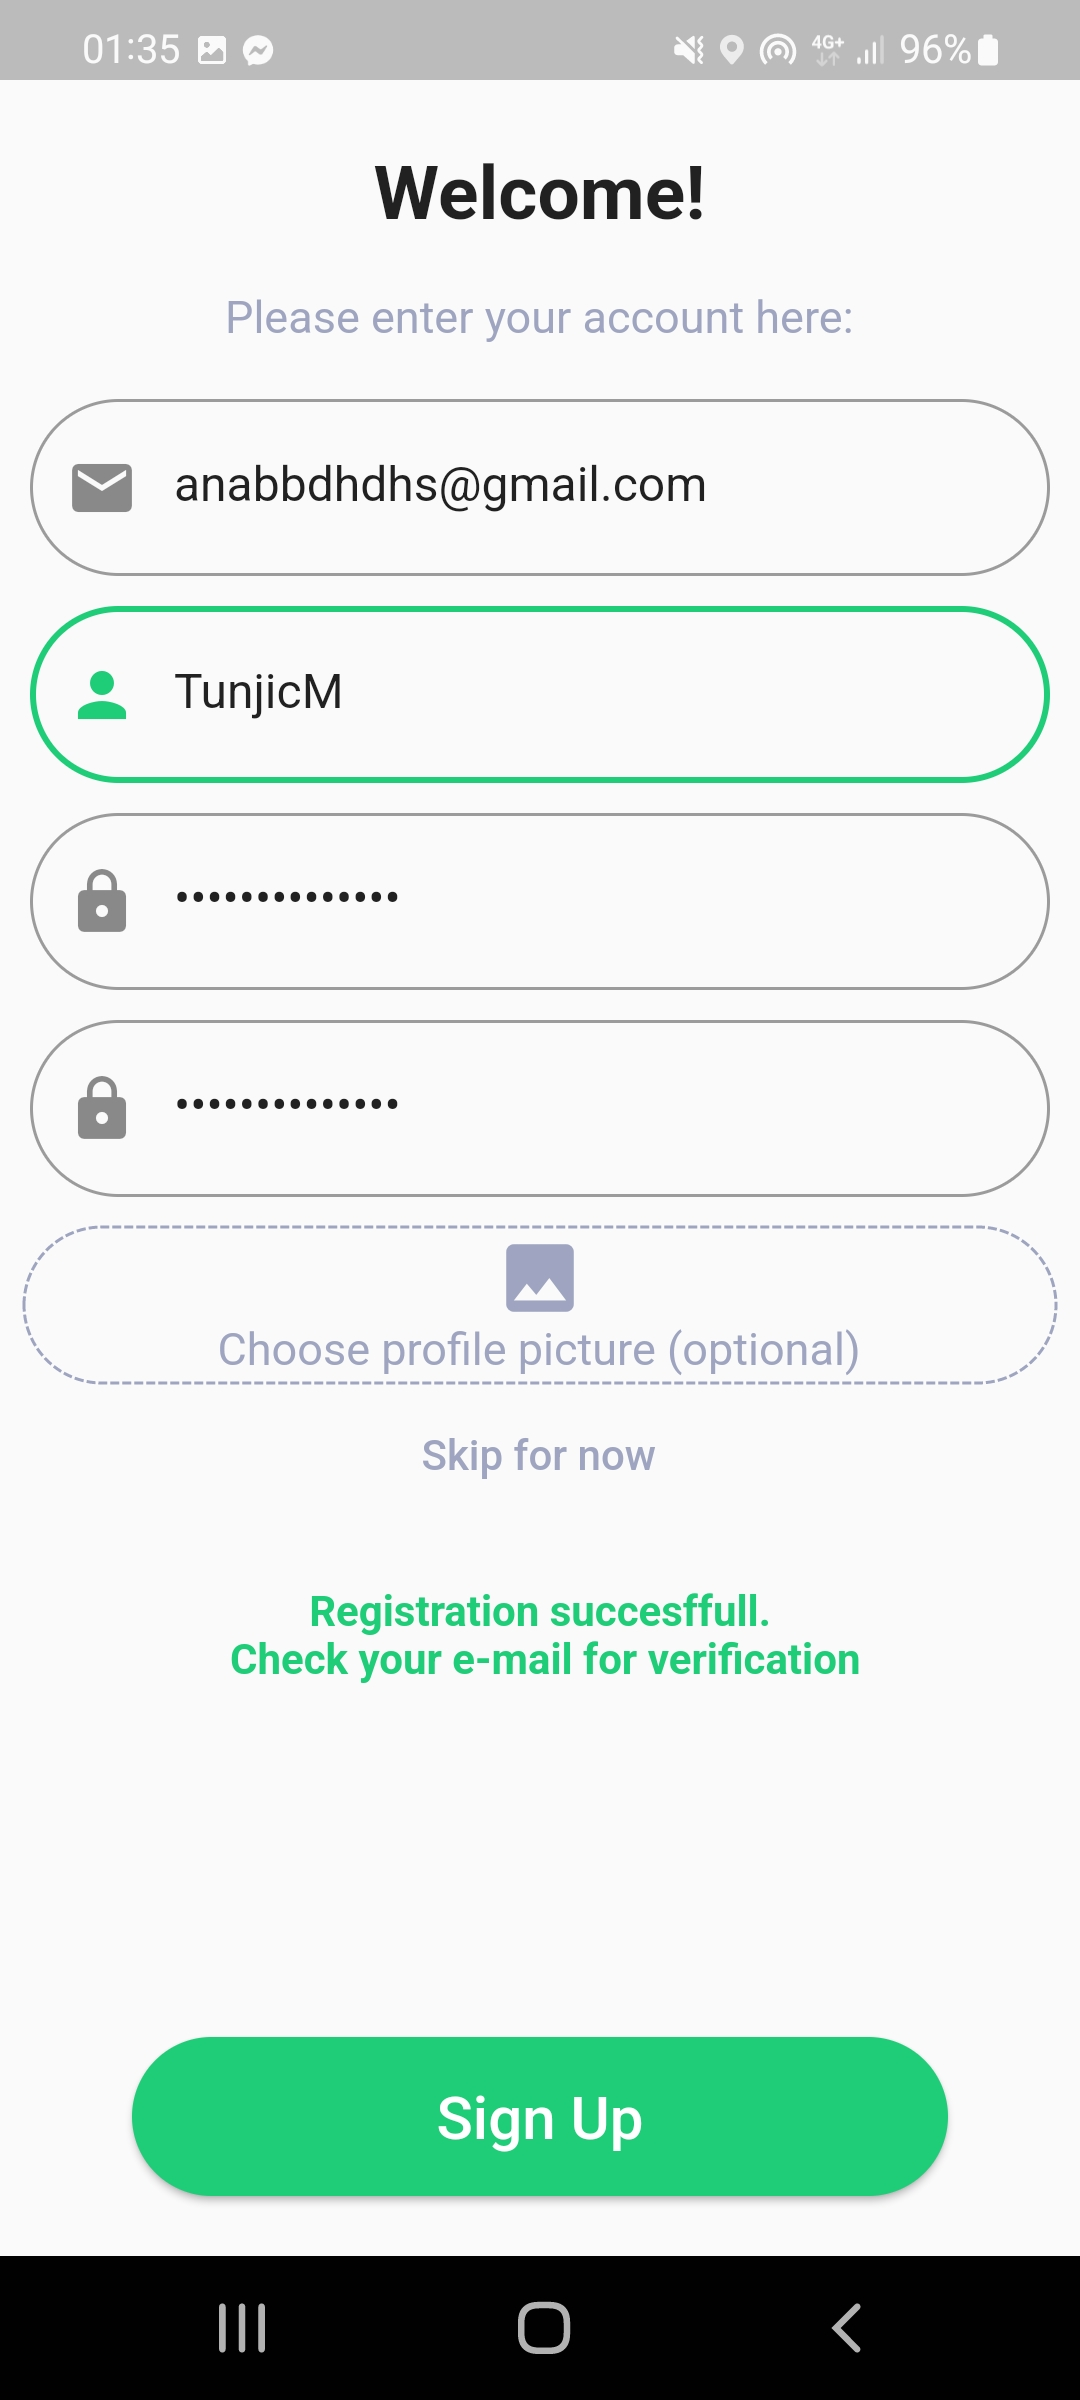
\includegraphics[width=.32\textwidth]{register_success.jpg} }}
      \subfloat[\centering Ekran za upravljanje korisnicima]{{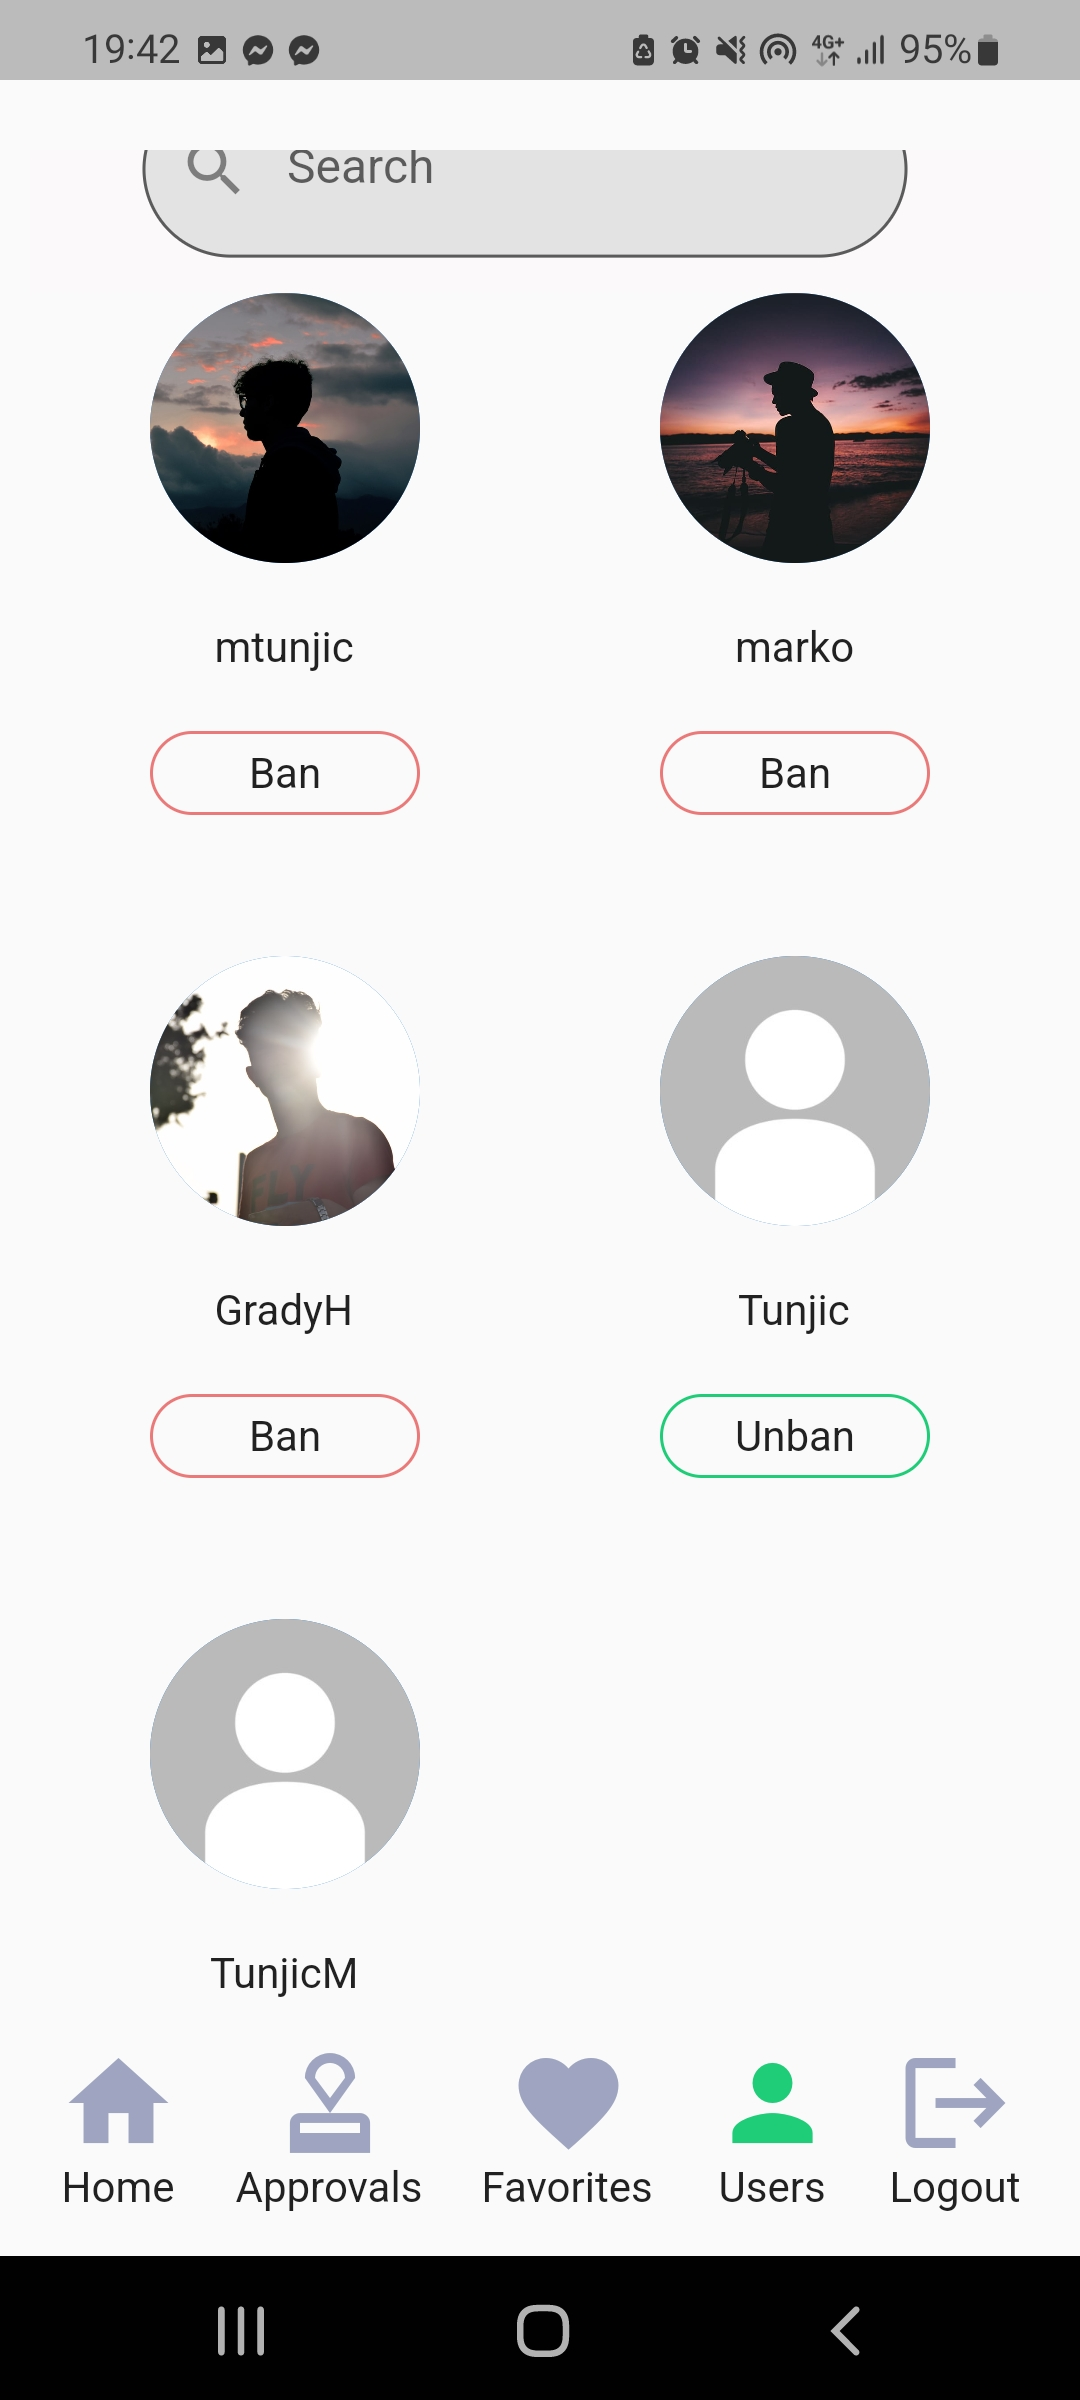
\includegraphics[width=.32\textwidth]{bans.jpg} }}
      \caption{Ekrani za registraciju i upravljanje korisnicima}
      \label{fig:Register}
\end{figure}

\subsection{Ekran za pregled svih recepata}
Ekran za pregled svih recepata će uvijek biti prvi ekran koji će se prikazati ako postoji
prijavljeni korisnik, a to se također postiže uz pomoć dijeljenih tajni \textit{(eng. SharedPreferences)}.
Estetski gledano ekran će biti jednak i za korisnike (prijavljene ili neprijavljene) i za administratore jedine dvije
razlike su u prikazu gumba za dodavanje u favorite i
u navigacijskoj traci, koja sadržava samo one gumbove koji vode do ekrana koji su dozvoljeni
trenutno prijavljenom to jest neprijavljenom korisniku (slika \ref{fig:All recipes}).
\\\\
U dijeljenje tajne se spremaju podatci o trenutnom korisniku kao na primjer: korisničko ime, identifikacijski
broj i \textit{JWT token} za autentifikaciju i autorizaciju.
To je bitno jer će se prije svakog upita, koji se obavlja daljnjom interakcijom
korisnika i aplikacije, u HTTP zaglavlje staviti spomenuti token uz pomoć kojeg će
poslužiteljska strana obaviti autentifikaciju i autorizaciju. Ako korisnik ne bude uspješno
autoriziran biti će odjavljen i preusmjeren na ekran za prijavu s odgovarajućom porukom.
\\\\
Na ovom ekranu moguće je vidjeti sve recepte koji sa nalaze u bazi podataka. Recepti su podijeljeni u stranice,
a svaka stranica sadrži 10 recepata, ako postoji više od 10 recepata na dnu ekrana će se pojaviti
jedan poseban \textit{widget} koji služi za prelazak na sljedeću, prethodnu ili neku određenu stranicu.
Svaki recept je opisan autorom i profilnom slikom autora, pozadinskom slikom recepta, nazivom,
prosječnom ocjenom i vremenom potrebnim za pripremu. Klikom na bilo koji opisnik recepta se otvara novi ekran,
a to je ekran za pregled pojedinog recepta. Na kraju postoji i gumb koji služi za brisanje recepta koji
je prikazan samo u slučaju da recept pripada trenutno prijavljenom korisniku ili je trenutno prijavljeni
korisnik zapravo administrator.
\\\\
Također na samom vrhu ekrana postoji \textit{widget} koji služi za filtriranje recepata po nazivu,
a pored njega se nalazi jedan gumb koji prilikom dodira otvara dijalog kojim
se mogu filtrirati recepti po sastojcima i vremenu pripreme.
\begin{figure}[h]
      \centering
      \subfloat[\centering Ekran sa svim receptima za neprijavljenog korisnika]{{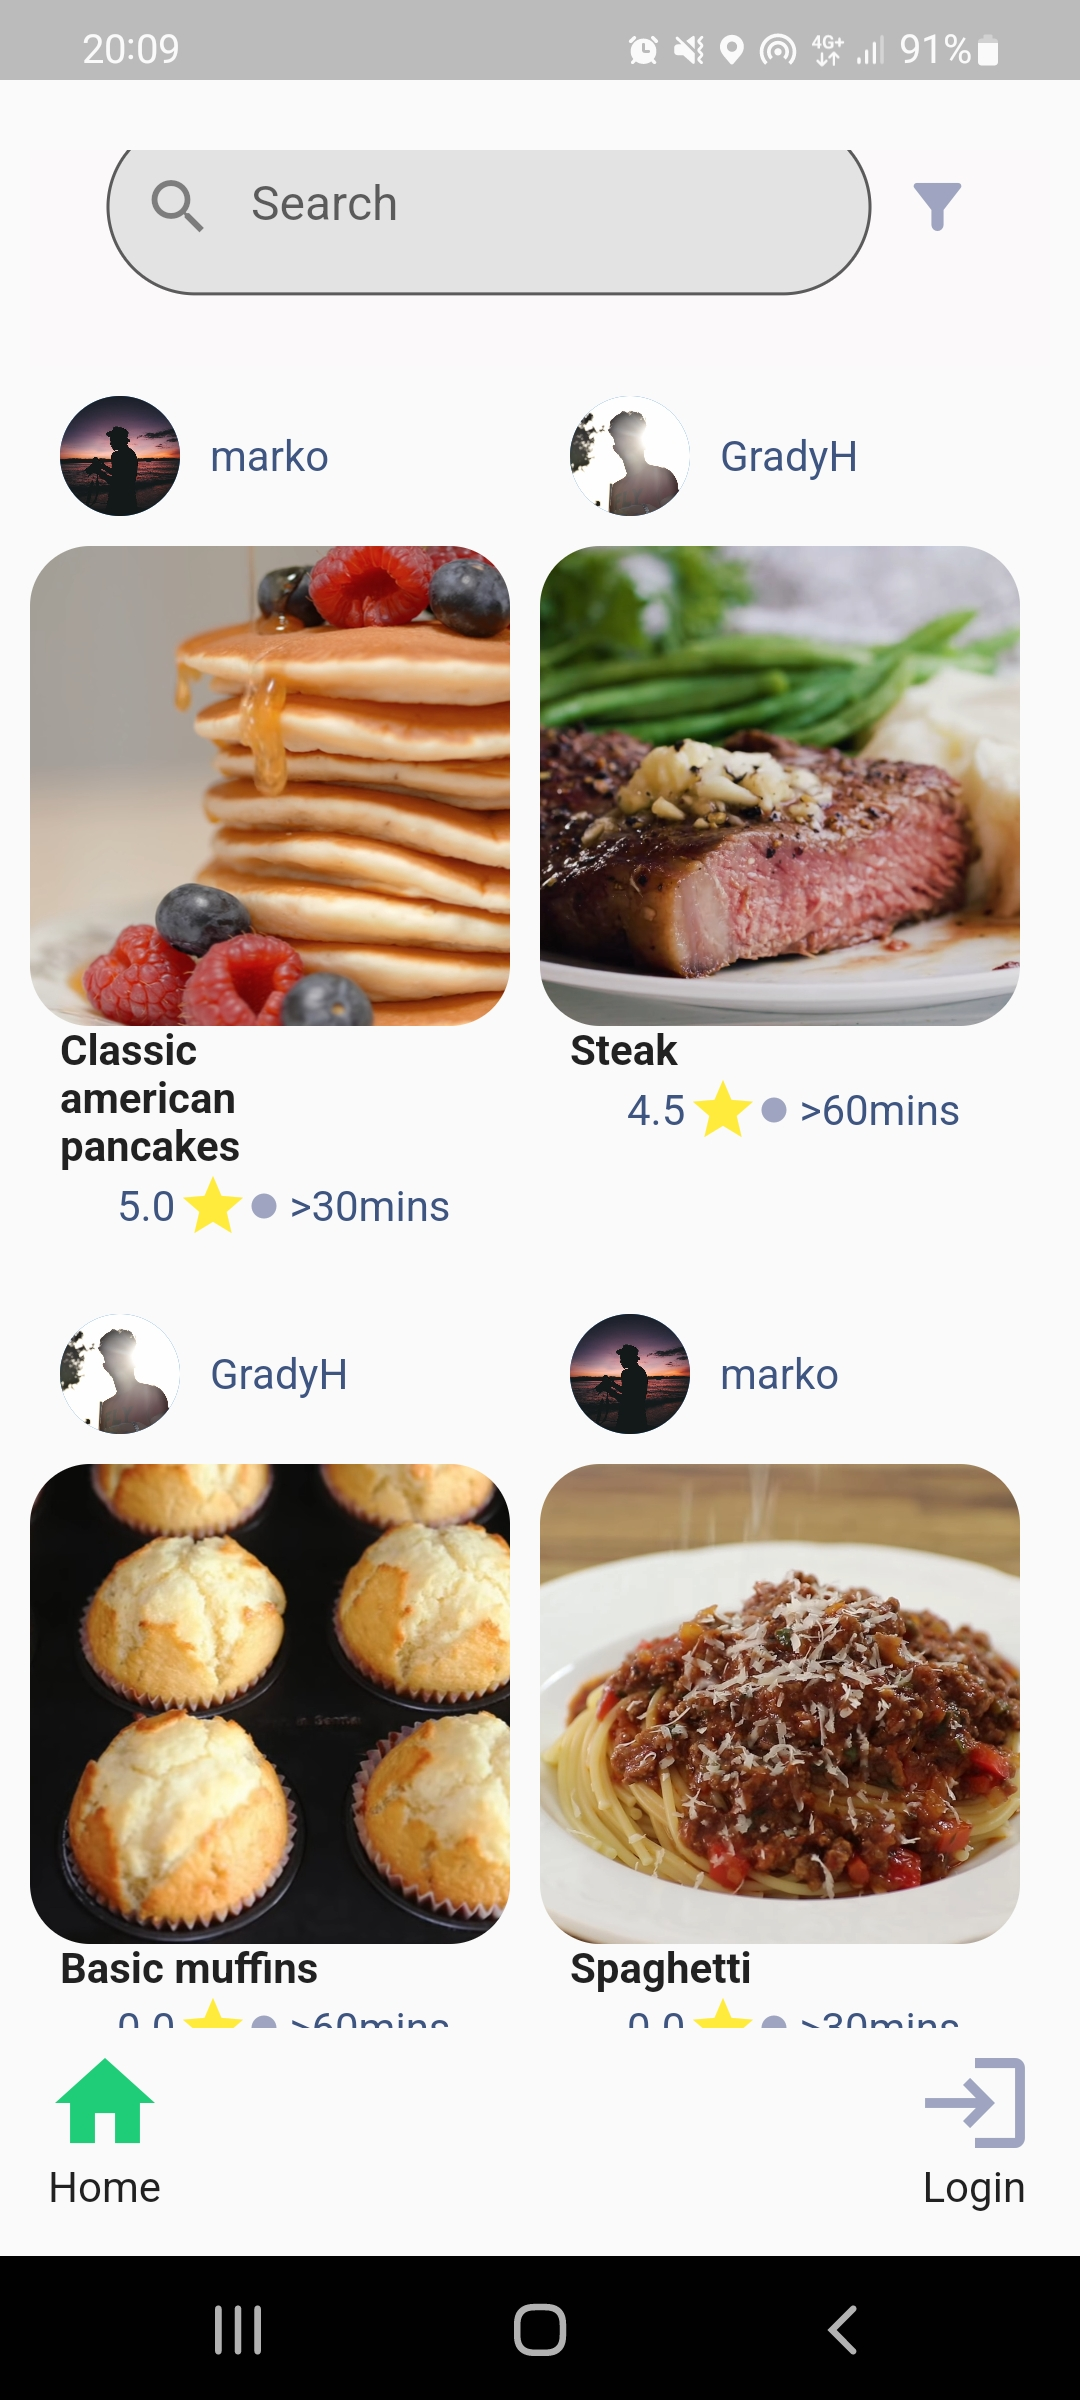
\includegraphics[width=.25\textwidth]{not_loggedin.jpg} }}
      \subfloat[\centering Ekran sa svim receptima za prijavljenog korisnika]{{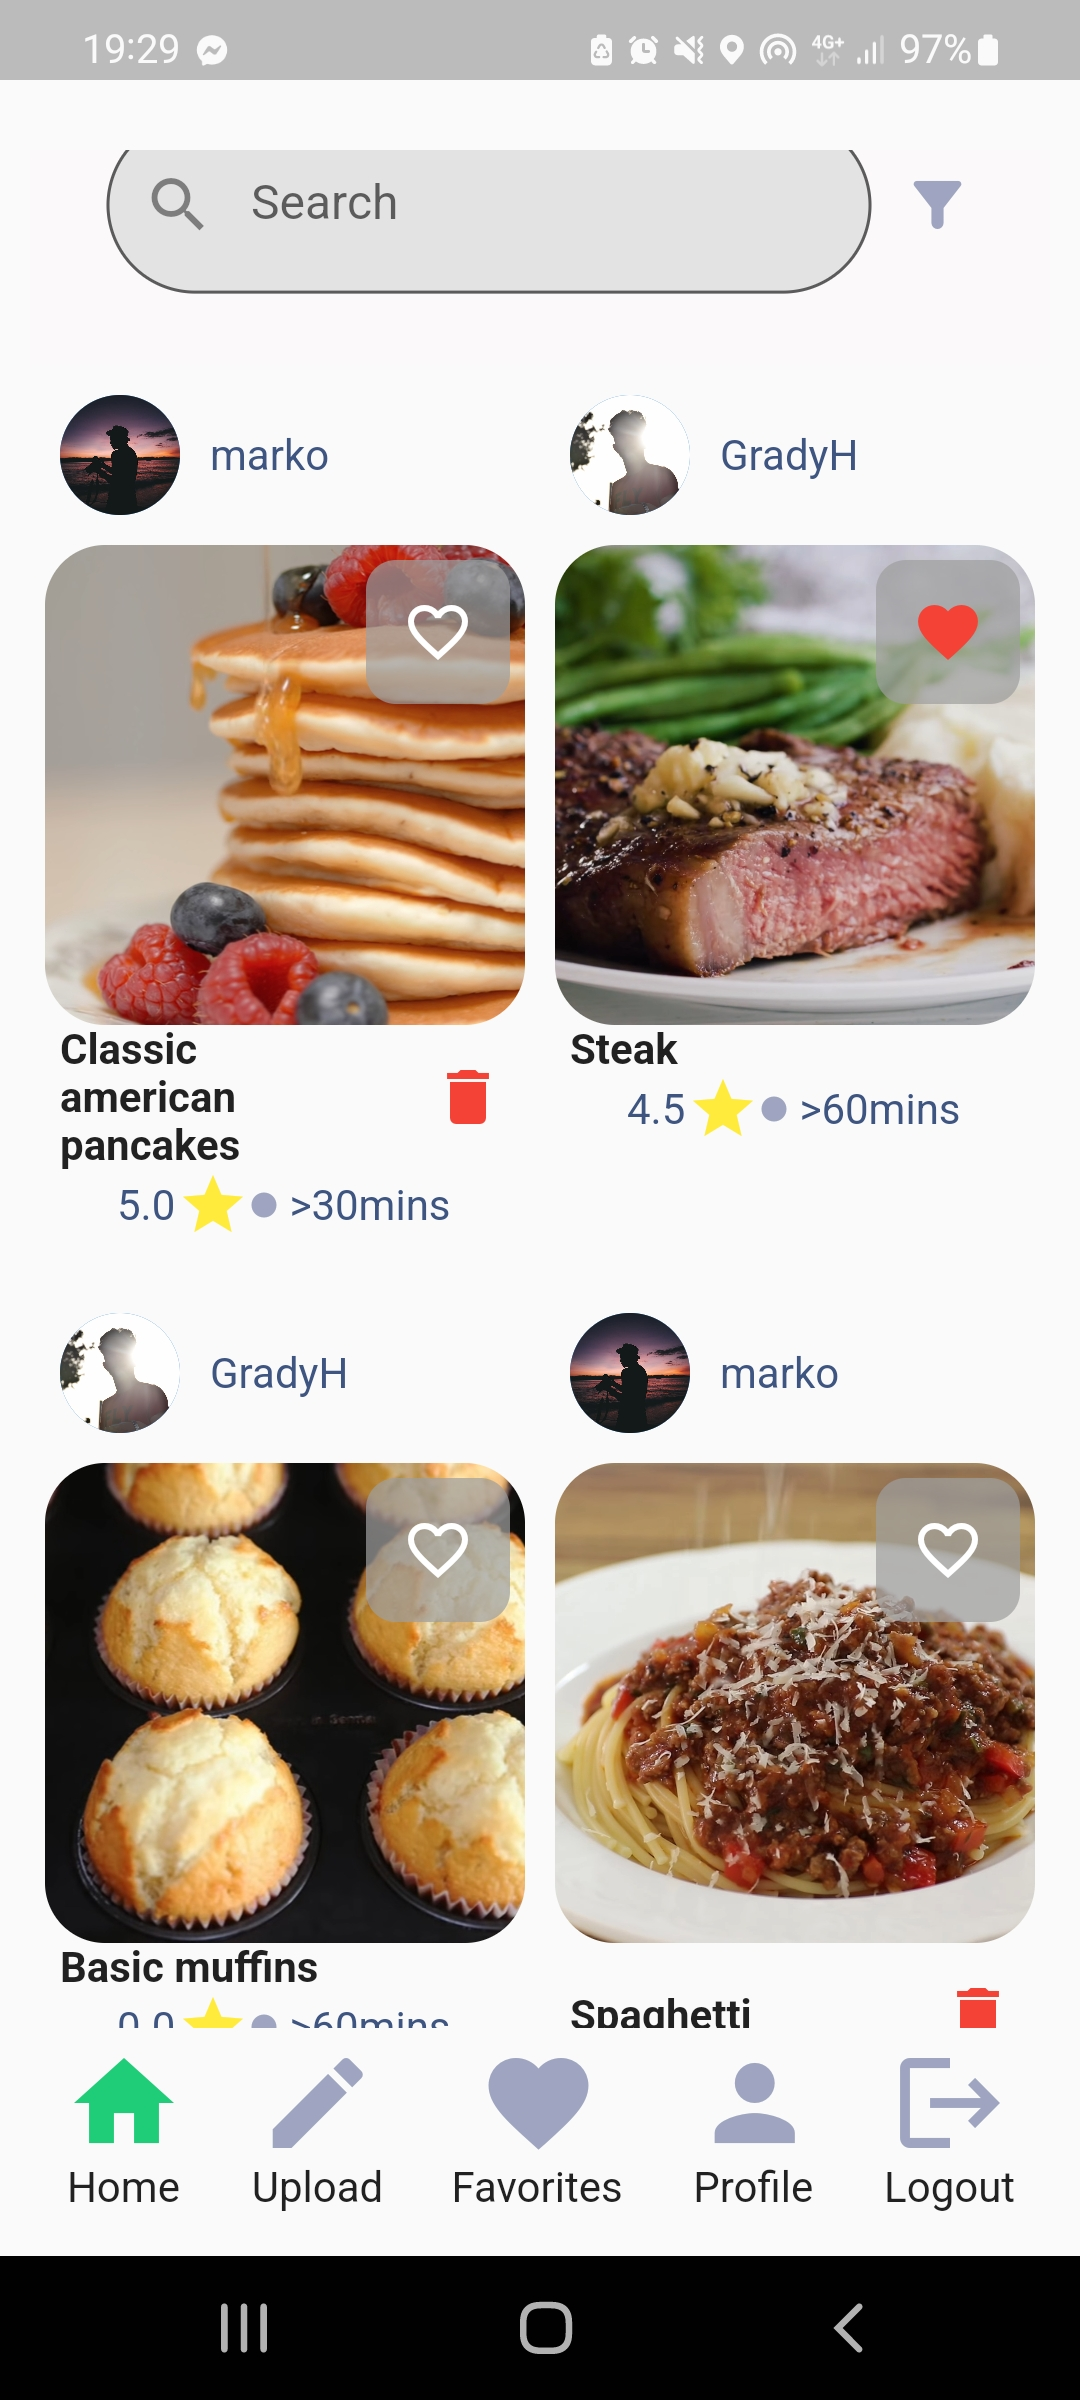
\includegraphics[width=.25\textwidth]{user_all_recipes.jpg} }}
      \subfloat[\centering Dijalog za filtriranje]{{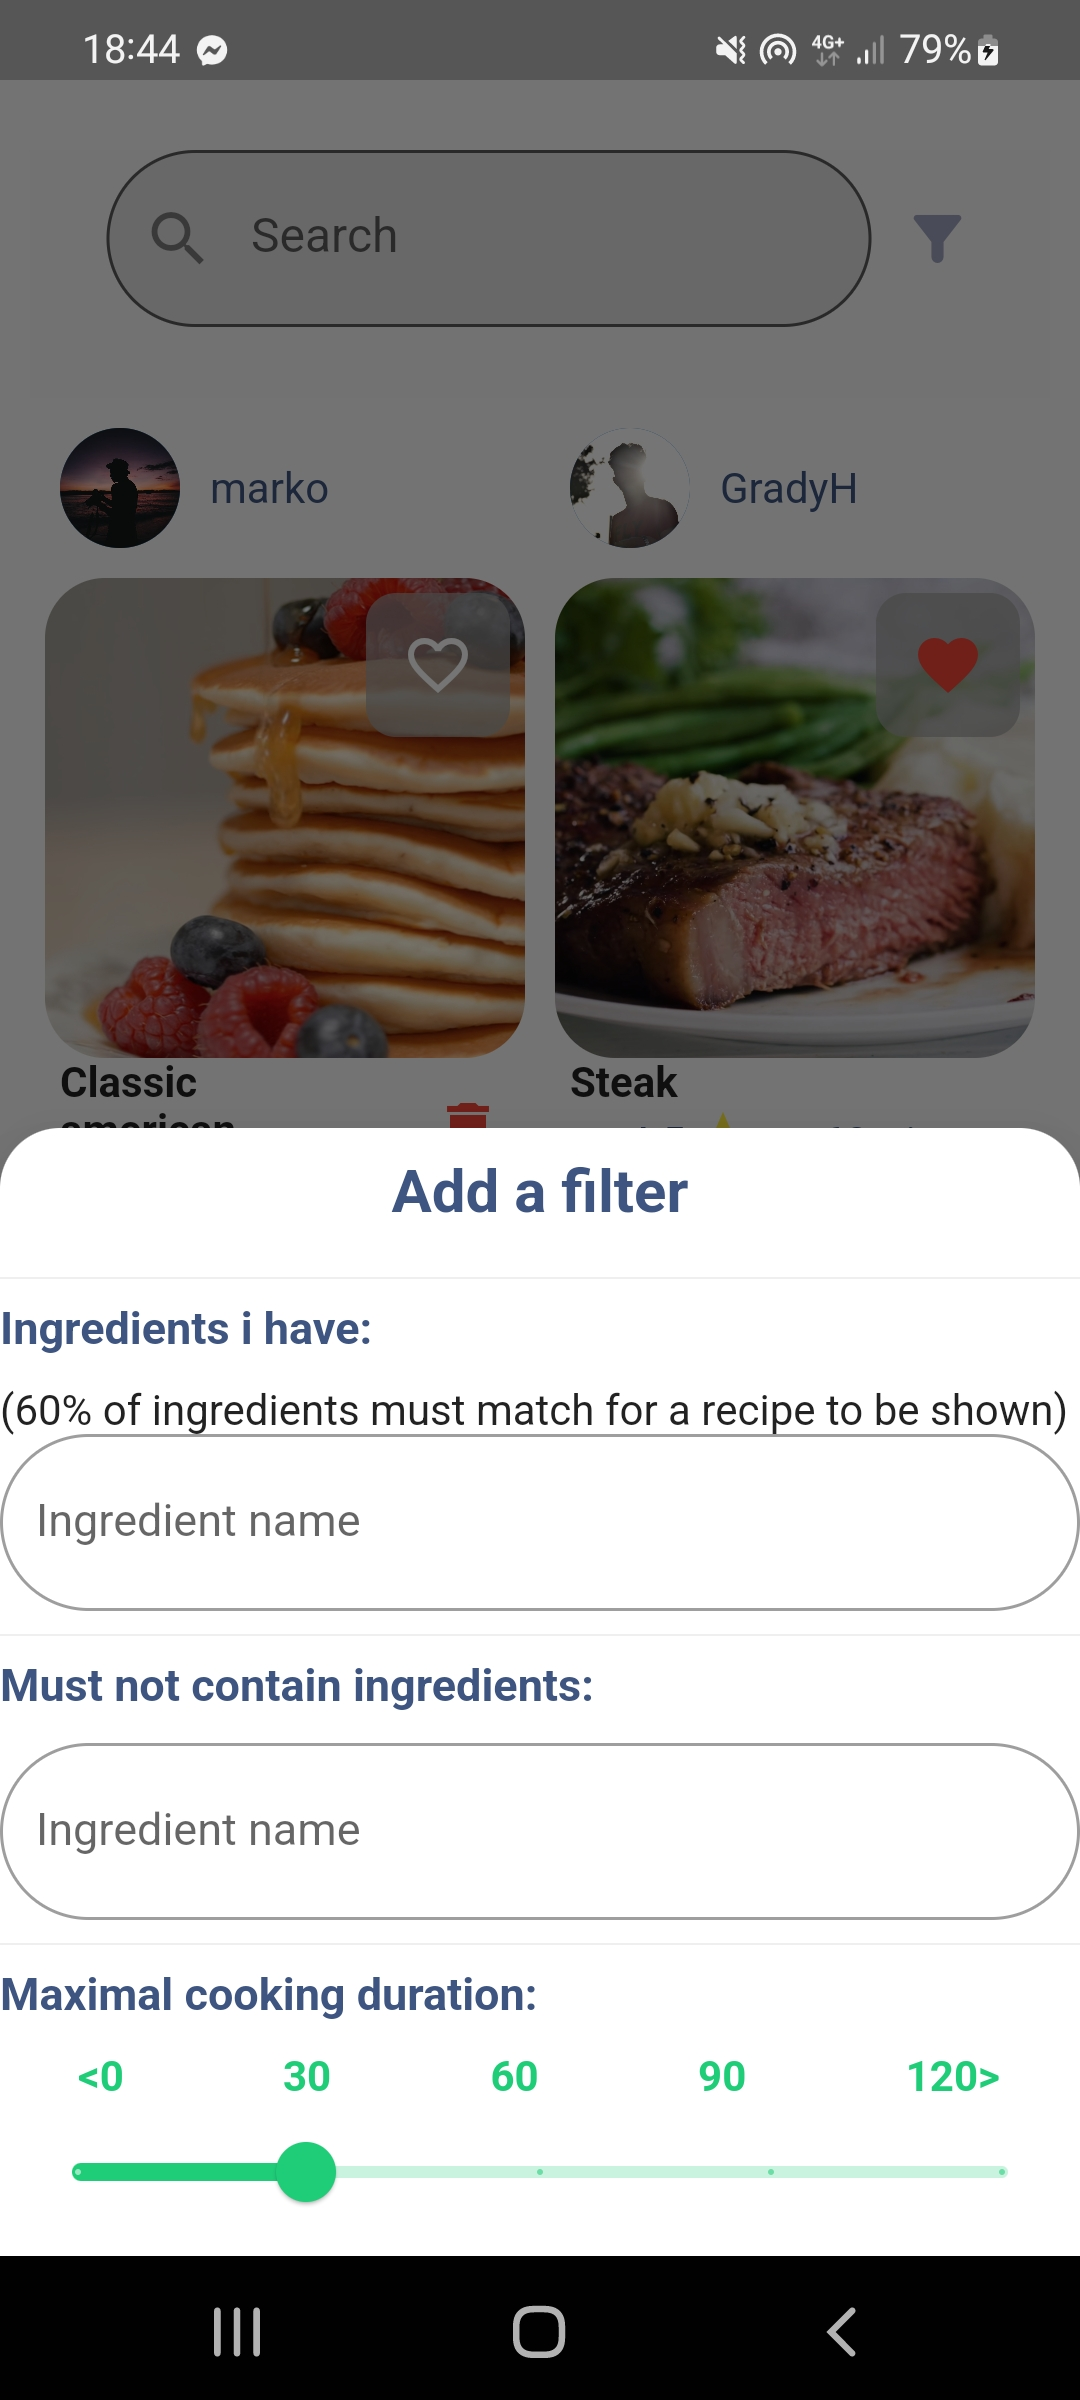
\includegraphics[width=.25\textwidth]{filter.jpg} }}
      \subfloat[\centering Ekran za odobravanje recepata]{{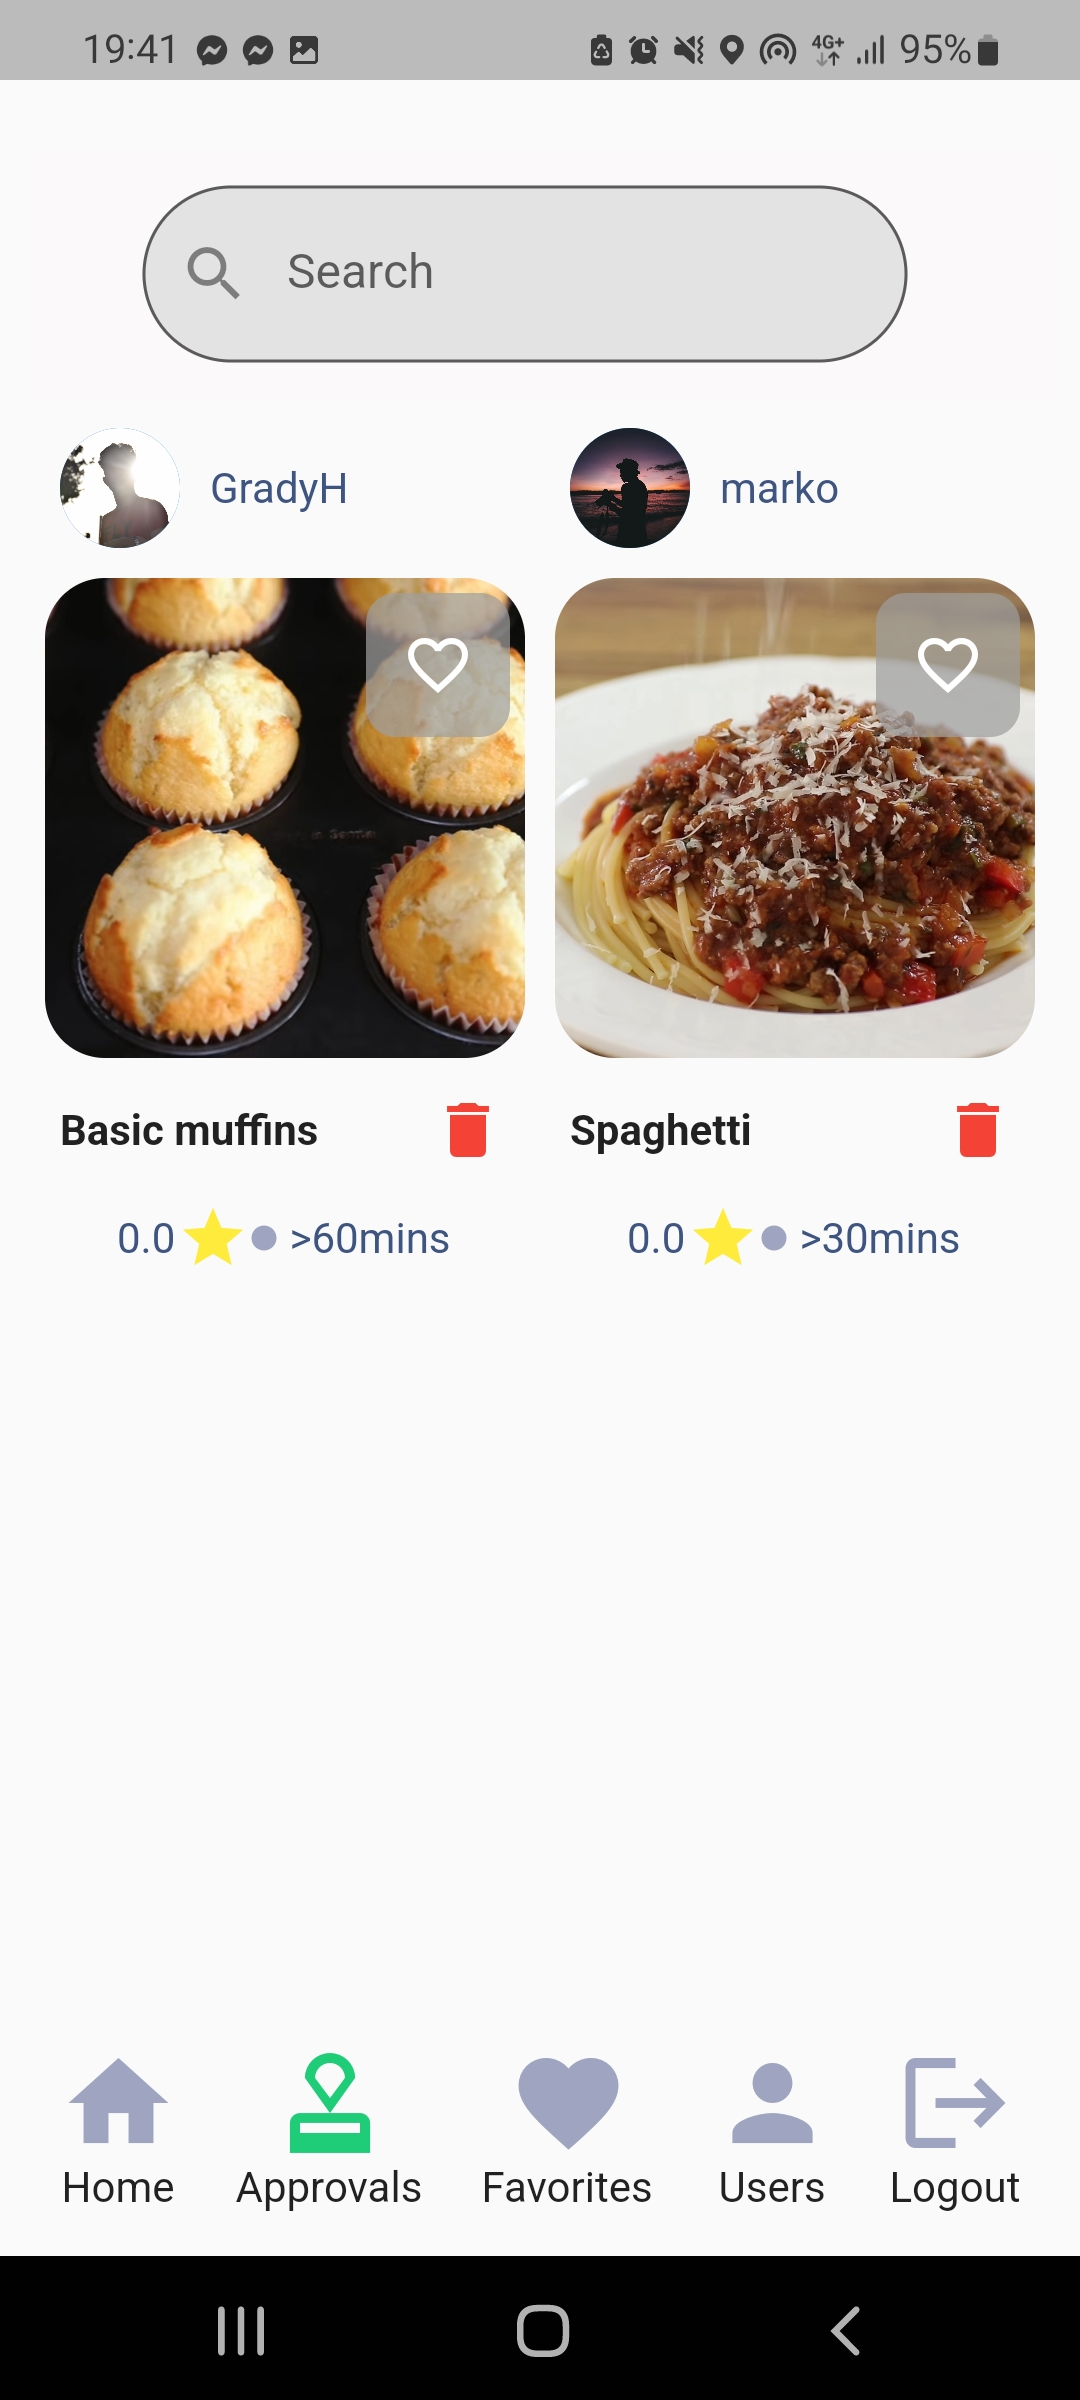
\includegraphics[width=.25\textwidth]{approovals.jpg} }}
      \caption{Ekrani sa receptima}
      \label{fig:All recipes}
\end{figure}

\subsection{Ekran za pregled pojedinog recepta}
Ekran za pregled pojedinog recepta će prikazivati sve podatke o receptu, a to su:
sastojci, koraci pripreme, svi videozapisi i fotografije
koje se nalaze u skrolabilnoj listi s kojom se interagira pokretima lijevo i desno, te dodatno ako
trenutno prijavljeni korisnik ima dovoljne ovlasti moći će interagirati s gumbom za ocjenjivanje i
poljem za unos komentara
\\\\
Ovaj ekran je također poprilično jednak i za obične korisnike i za administratore,
sa razlikom da administratori imaju pristup gumbu za odobravanje ili onemogućavanje recepta, a neprijavljeni
korisnici nemaju pristup gumbu za ocjenjivanje i komentiranje (slika \ref{fig:Single recipe} (c) i (d)).
\begin{figure}[h]
      \centering
      \subfloat[\centering Prvi dio ekrana za dodavanje recepta]{{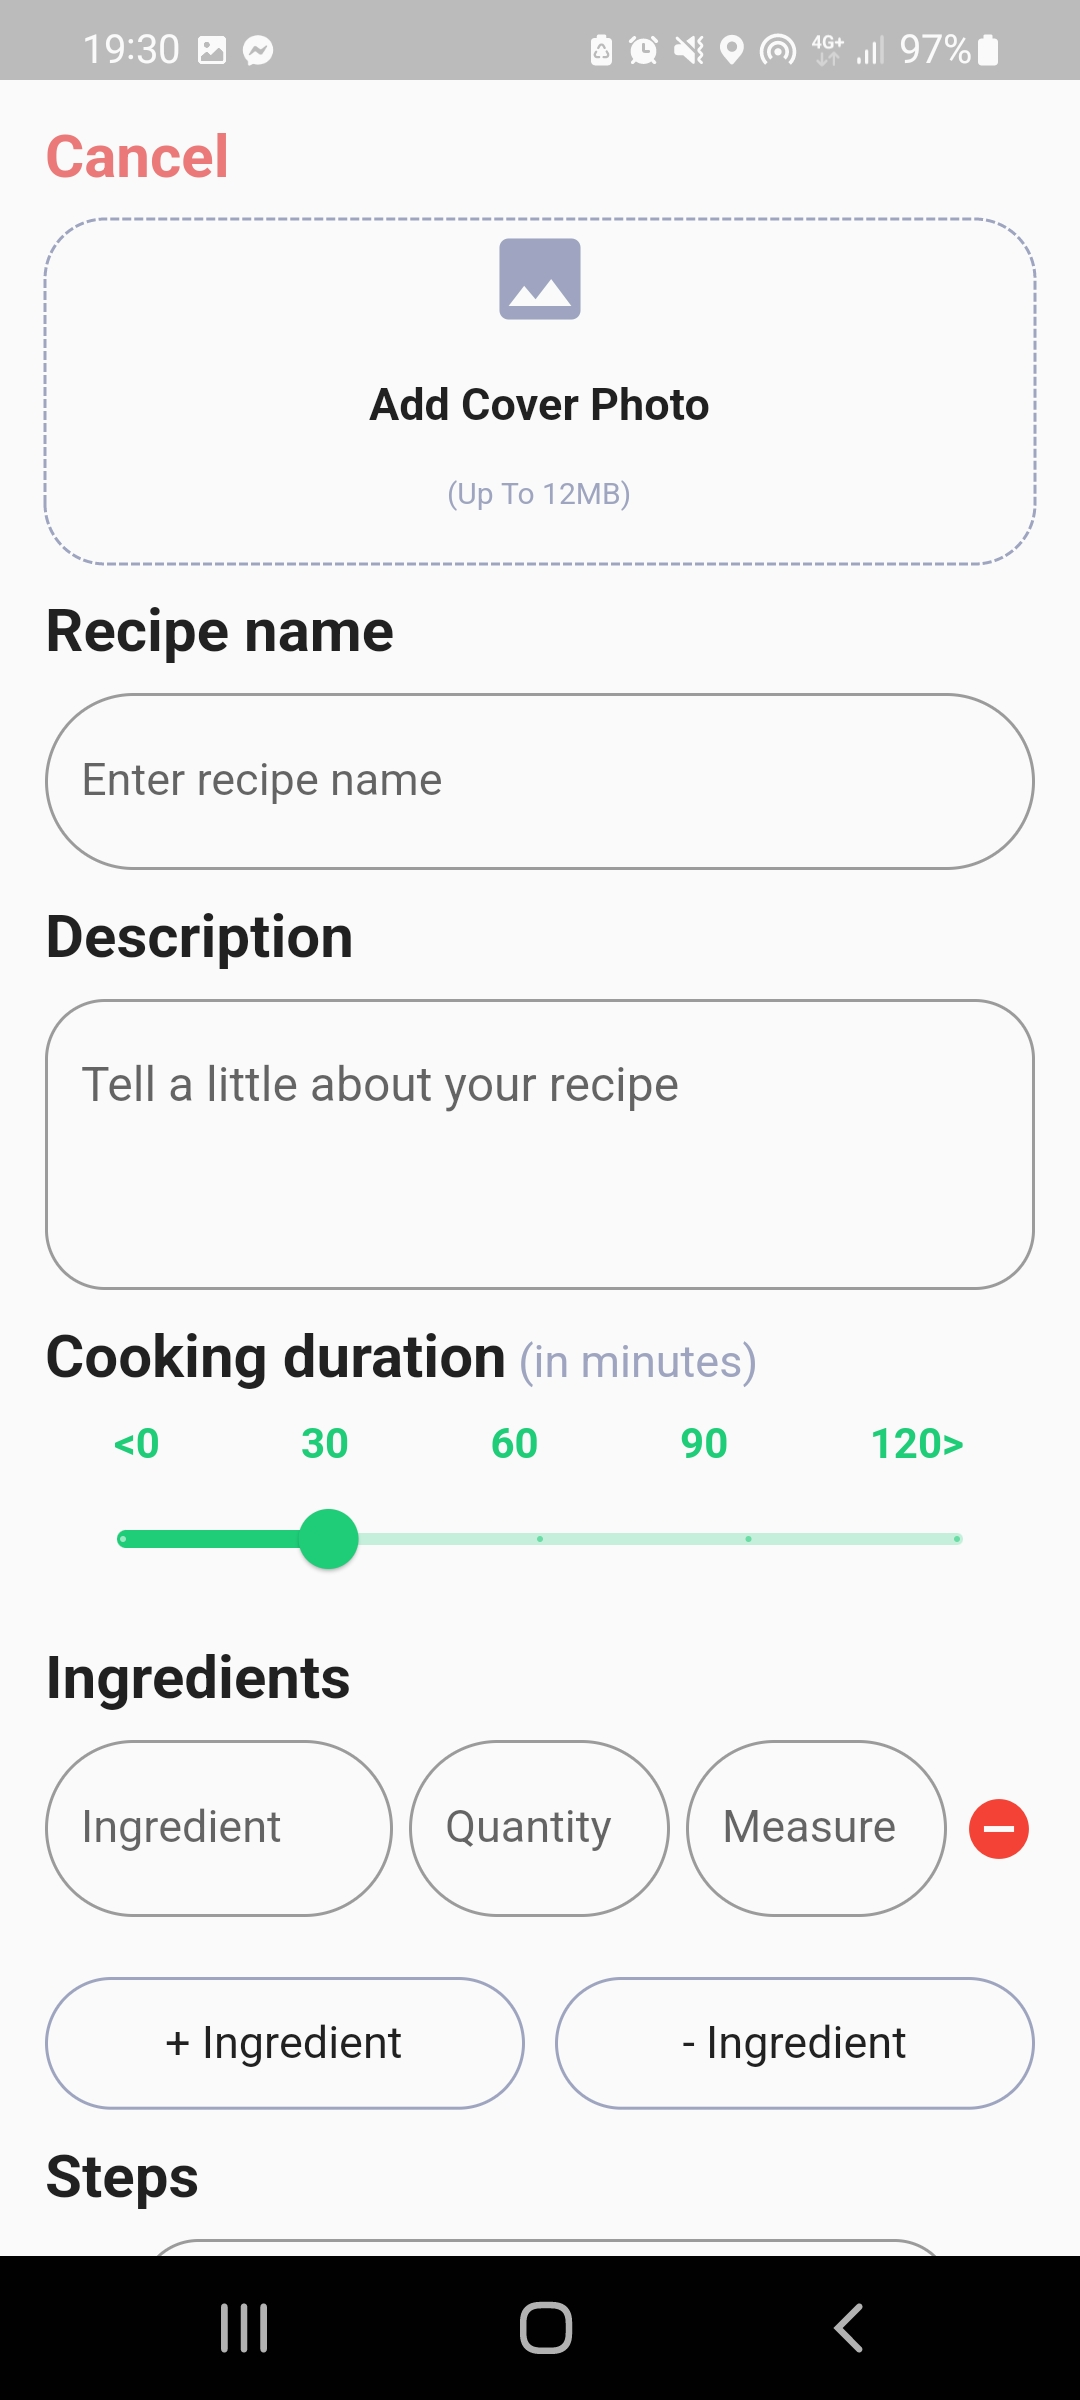
\includegraphics[width=.25\textwidth]{new_recipe1.jpg} }}
      \subfloat[\centering Drugi dio ekrana za dodavanje recepta]{{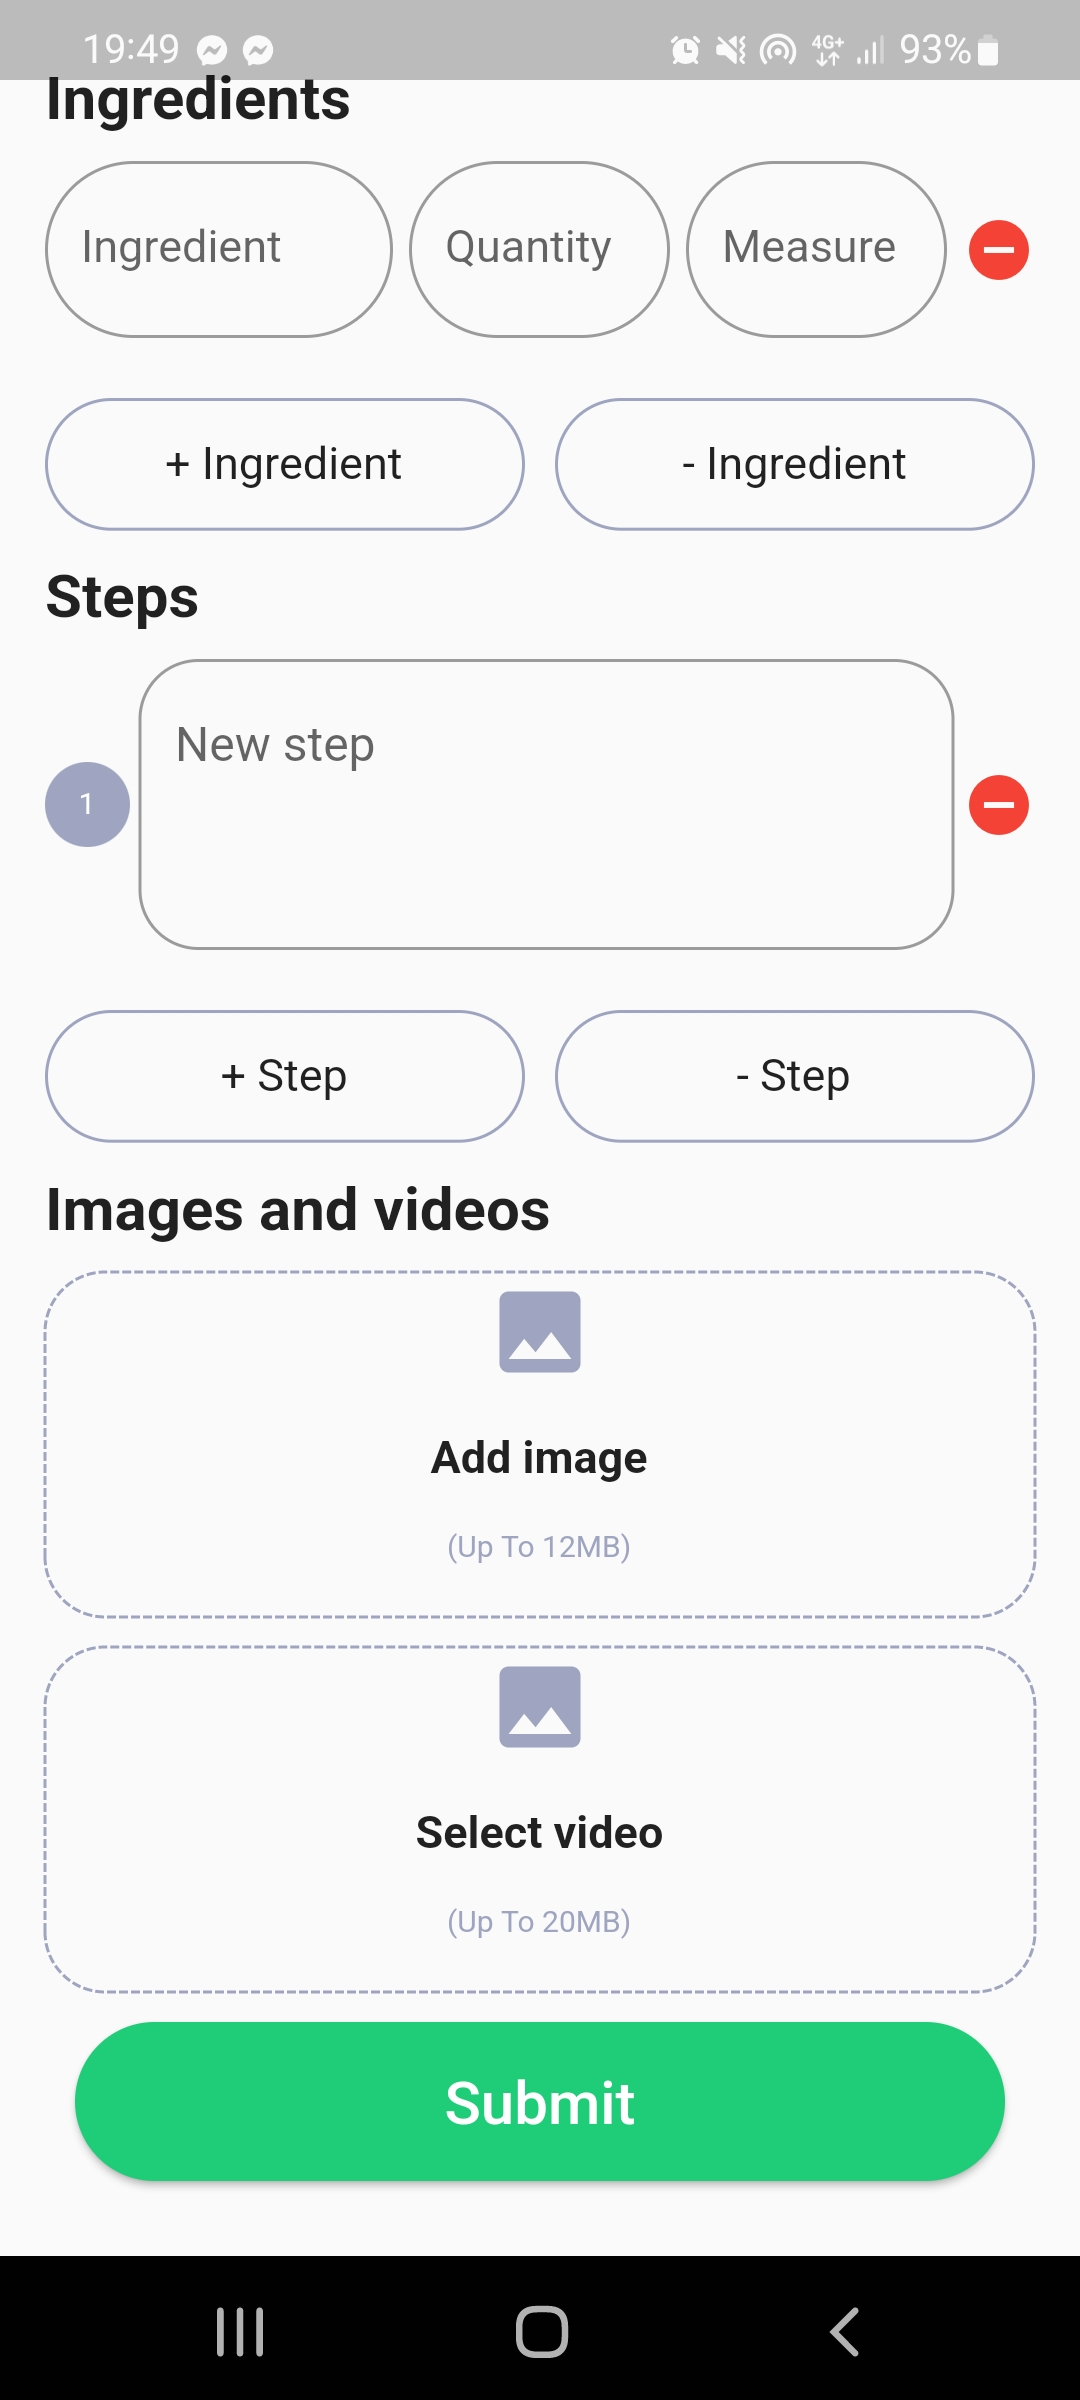
\includegraphics[width=.25\textwidth]{new_recipe2.jpg} }}
      \subfloat[\centering Prvi dio ekrana za detalje o receptu]{{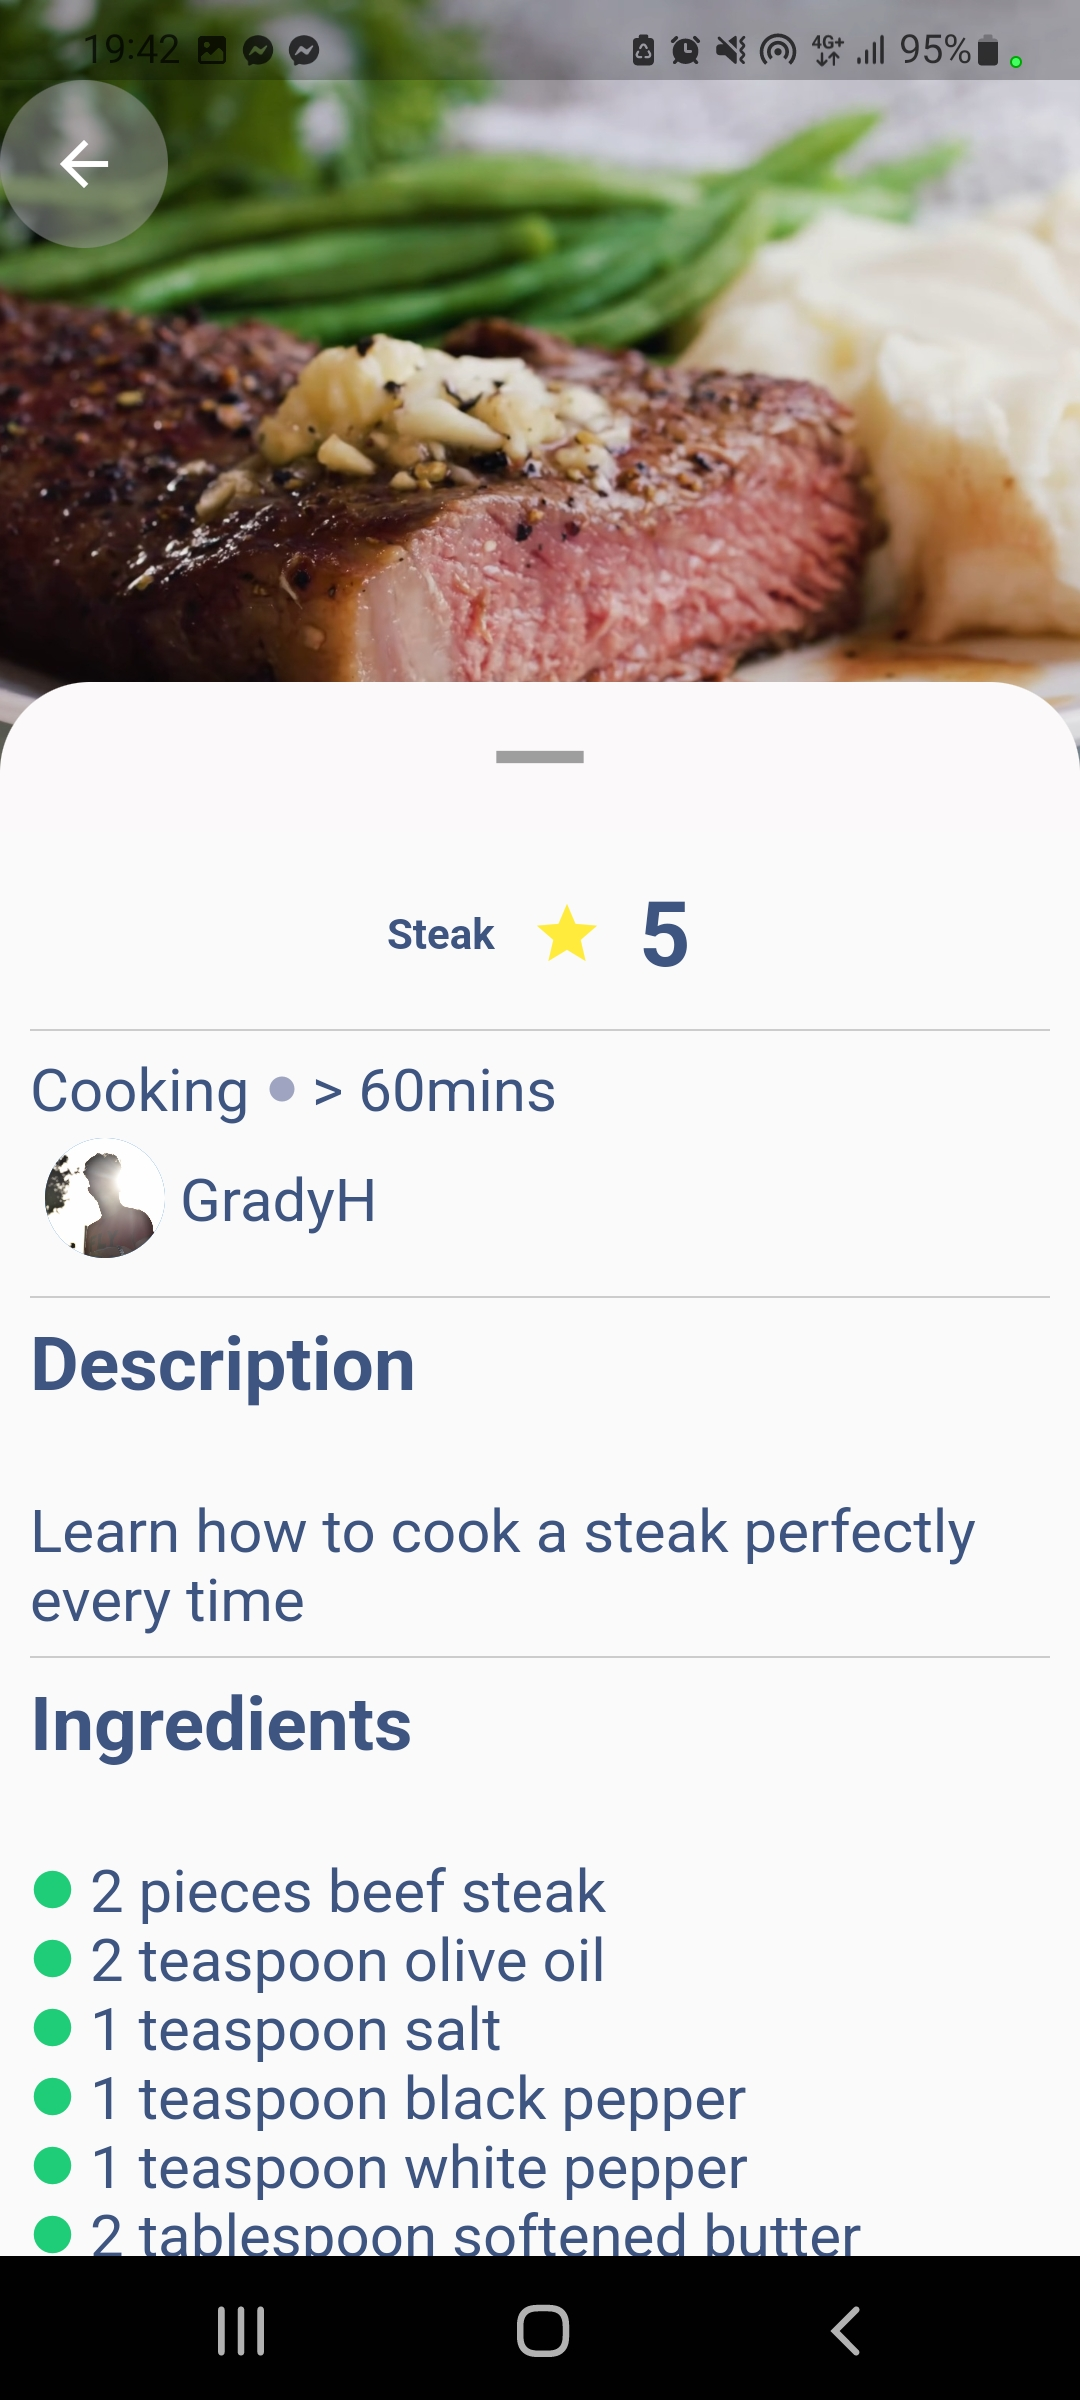
\includegraphics[width=.25\textwidth]{single_recipe_user.jpg} }}
      \subfloat[\centering Drugi dio ekrana za detalje o receptu]{{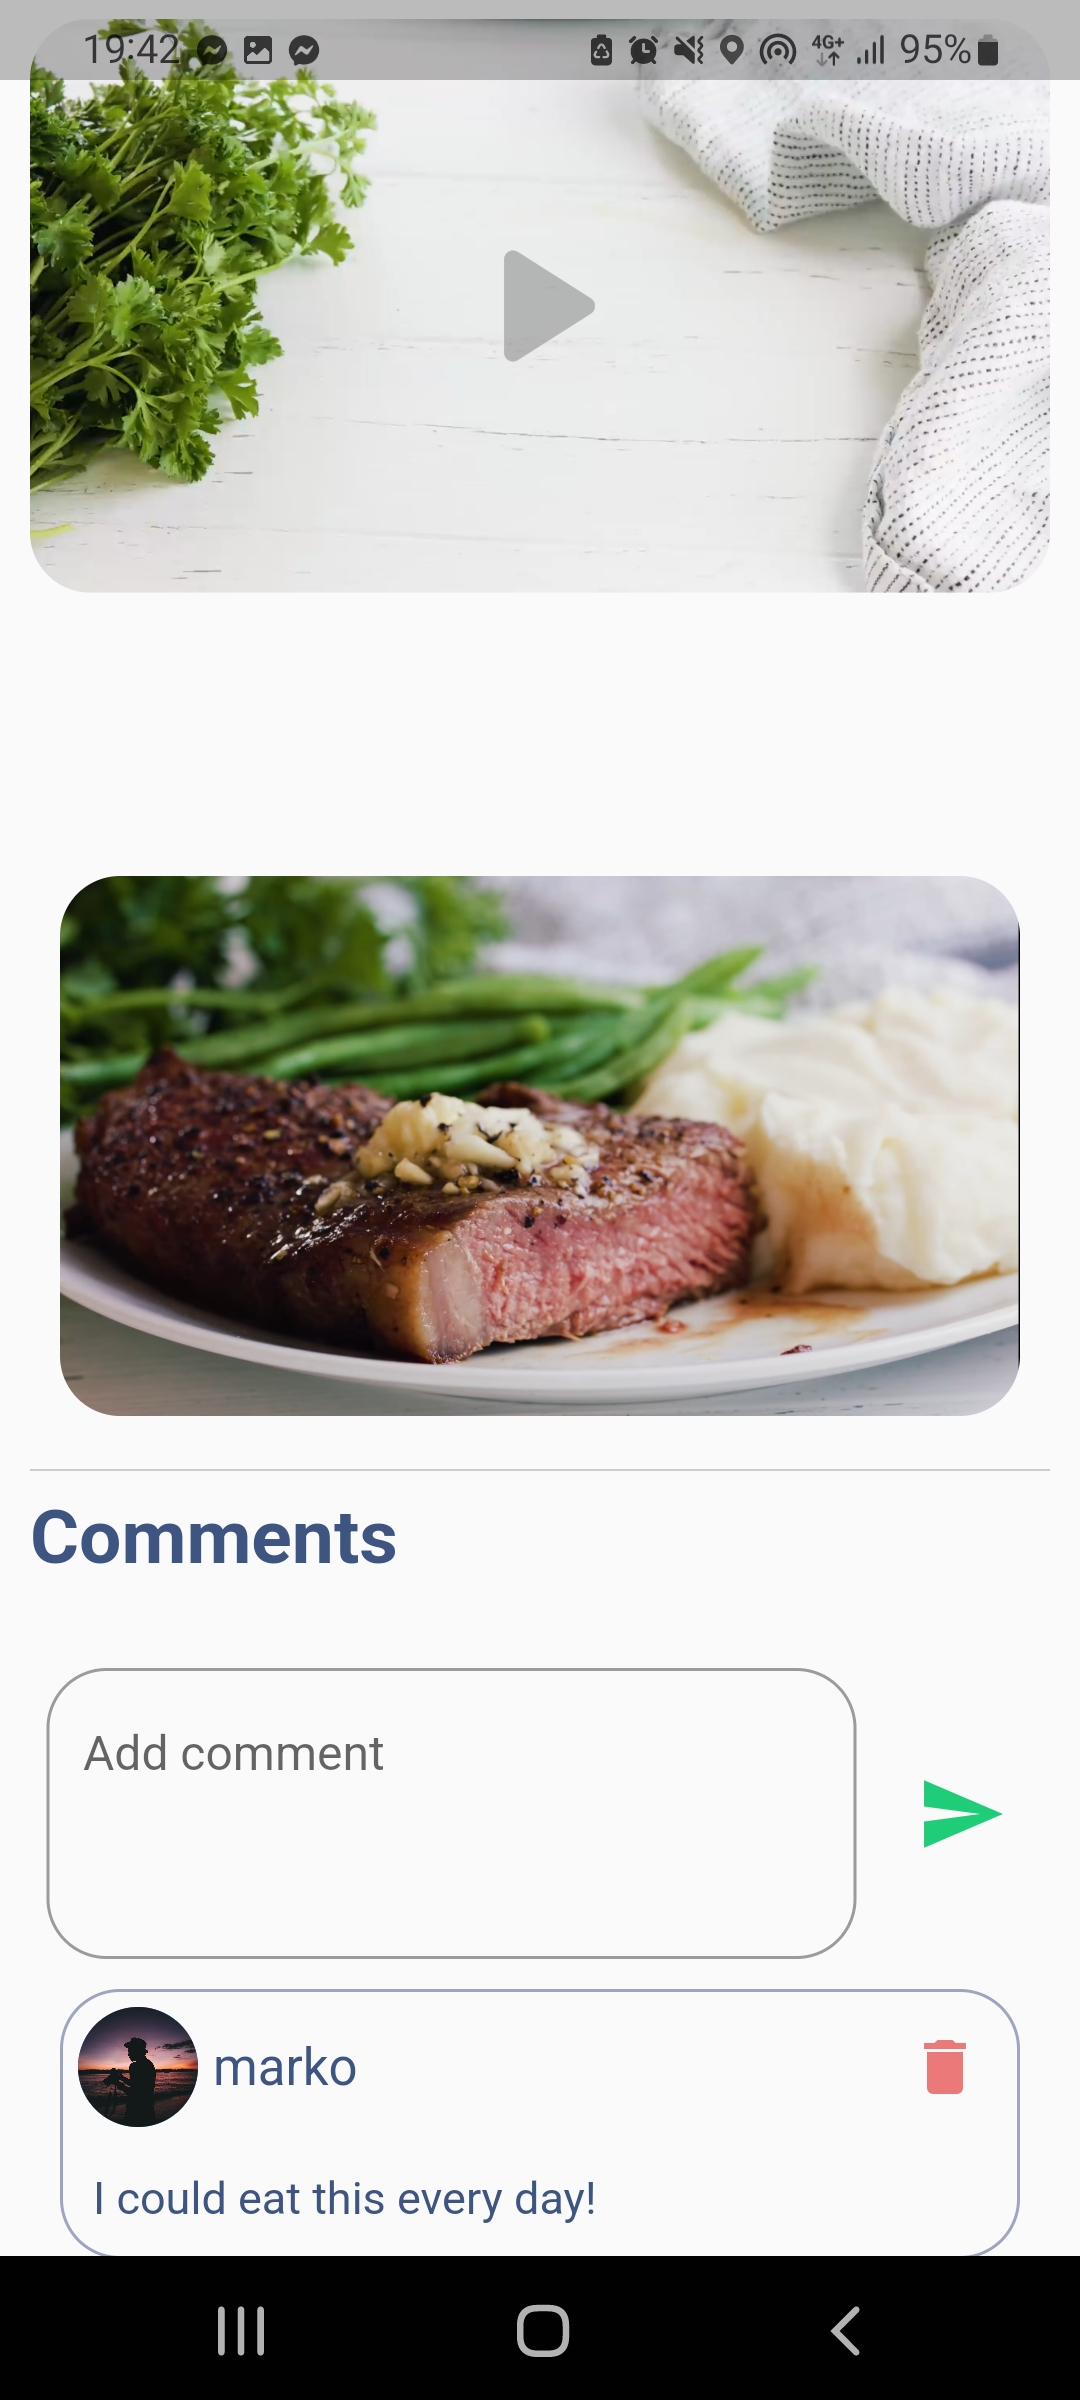
\includegraphics[width=.25\textwidth]{images_videos_comments.jpg} }}
      \caption{Ekrani za pojedini recept}
      \label{fig:Single recipe}
\end{figure}

\subsection{Ekran za dodavanje novog recepta}
Ekran za dodavanje novog recepta je dostupan samo prijavljenim korisnicima koji nisu administratori.
Ovaj ekran se sastoji od velikog broja polja za unos i odabir videozapisa i fotografija te gumba za potvrdu.
Karakteristika svakog polja je da ne smije biti prazno i ne smije sadržavati više znakova od broja koji
je određen bazom podataka. Posebne sekcije su sekcije za unos sastojaka, koraka pripreme, videozapisa i
fotografija jer su sve te sekcije modelirane BLoC obrascem jer nije moguće unaprijed znati koliko
takvih objekata korisnik želi dodati pa je bilo potrebno dodati opciju za dinamičko dodavanje
polja za unos (slika \ref{fig:Single recipe} (a) i (b)).

\subsection{Ekran za upravljanje korisnicima}
Posljednji ekran je ekran za upravljanje korisnicima, one je dostupan samo administratorima. Na ovoj stranici se
nalazi popis svih korisnika koji su također podijeljeni u stranice gdje svaka stranica sadrži 10 korisnika
i straničenje funkcionira na potpuno jednak način kao i straničenje za recepte.
Jedan korisnik je opisan svojim korisničkom imenom profilnom slikom i gumbom za suspendiranje to jest
odsuspendiranje korisnika. Nema opcije za brisanje korisnika jer bi to značilo da bi pojedini recepti
ostali bez autora ili bi bili obrisani iz baze što nije poželjna funkcionalnost. Zato je korinsiku
samo onemogućena prijava u sustav (slika \ref{fig:Register} (c)).

\chapter{Zaključak}
Mobilne aplikacije su postale važan dio modernog društva. Iz tog razloga ih je potrebno napraviti što je
bolje moguće. Za takve svrhe postoje razni obrasci, načela programiranja, stilovi i tehnike: neke od
korištenijih su MVC obrazac, podjela na poslužiteljsku stranu, korisničku stranu i bazu podataka,
native pristup razvoju aplikacija, oblak, GraphQL stil i slično.
\\\\
Najbitnija stvar je da krajnji korisnik bude zadovoljan, a to se postiže uz ergonomski dizajn aplikacije,
brzinu i sigurnost. Zato postoje alati kao na primjer: flutter uz pomoć kojeg se bez većih problema razvije aplikacija koja
je laka za koristiti, ili SpringBoot s kojim se lako implementira sigurnost i podjela uloga, ili GraphQL koji
nudi brzinu i optimalnost aplikacije te oblak uz pomoć kojeg sve postaje javno dostupno.

\bibliography{literatura}
\bibliographystyle{fer}
\nocite{ProgramiranjeUJavi}
\nocite{GraphQL}
\nocite{Authentication}
\nocite{Spring}

\begin{sazetak}
      Mobilne aplikacije su danas vrlo popularna stvar i u posljednje vrijeme popularnost sve više raste.
      Uzrok tomu je brzina i lakoća korištenja u usporedbi za klasičnim web aplikacijama. Iako su mobilne
      i web aplikacije u puno stvari slične kao na primjer MVC obrazac ili razdvajanje na poslužiteljsku i
      korisničku stranu, isto tako postoji i puno razlika a neke su napuštanje SOAP protokola u mobilnim
      aplikacijama, odsutnost sjednica, različiti jezici i radni okviri na korisničkoj strani i slično.
      \\\\
      Kao zamjena za SOAP protokol se vrlo često koristi REST arhitekturni stil, ali postoje i različiti
      stilovi kao na primjer GraphQL. GraphQL predstavlja stil u kojem se korisničkoj strani dopušta
      potupuna sloboda u biranju podataka, njihovom formatu i obliku. Njegova karakteristika je što
      rješava problem dohvata previše podatak, problem dohvata premalo podataka, problem velikog broja
      završnih točki na poslužitelju\dots U spring boot radnom okviru se GraphQL vrlo lako implementira uz
      pomoć ovisnosti prema graphql-spring-boot-starter i graphql-java-tools. Naime potrebno je samo definirati
      shemu i napraviti takozvane resolvere.
      \\\\
      Sada zbog GraphQL-a korisnička strana vrlo lako dohvati podatke koji su joj potrebni. Na primjer
      u flutter radnom okviru uz pomoć paketa flutter-graphql koji sadrži \textit{widget-e} koji su
      zaduženi za komunikaciju sa graphql poslužiteljem. Također GraphQL dopušta komunikaciju uz pomoć tokena
      pa je tako uz na primjer \textit{JWT token} vrlo lako obaviti autorizaciju i autentifikaciju te spremiti
      taj token u dijeljene tajne i na uz pomoć njega obaviti filtriranje ekrana koje trenutni korisnik smije
      vidjeti.
      \\\\
      \kljucnerijeci{Mobilna aplikacija, baza podataka, poslužiteljska strana, korisnička strana, oblak, PostgreSQL, SpringBoot, GraphQL, Flutter, Native, AWS .}
      \\\\\\\\
\end{sazetak}
% TODO: Navedite naslov na engleskom jeziku.
\engtitle{Mobile application for recipe managment}
\begin{abstract}
      Mobile applications are a very popular thing nowadays and since the past few years the popularity has
      grown by quite a lot. That is becouse they are very easy to use and very fast in comparison with
      web applications. Web and mobile applications have a lot in common like: MVC pattern or splitting
      the application on the database, backend, frontend, but they also have some differences like the
      absence of SOAP protocol in mobile applications, no sessions in mobile applications, different
      coding languages and frameworks on the frontend and so on.
      \\\\
      A commonly used substitute for the SOAP protocol is the REST architetural style, but there are some other
      options like GraphQL. GraphQL is a style that allows the frontend do define which data to fetch
      and in which shape and form. Its characteristic is that it solves the problem of overfetching, underfetching,
      then the problem of lot of endpoints\dots In the SpringBoot framework the GraphQL functionality
      is very easily implemented with the graphql-spring-boot-starter and graphql-java-tools dependency.
      The only thing that is neccessary is a schema and some resolvers.
      \\\\
      Now becouse of GraphQL the frontend can fetch the neccessary data without any problems. For example
      in the flutter framework with the help of flutter-graphql package that contains widgets that
      are used for communication with a GraphQL server. Also GraphQL allows communications with tokens
      so it is possible to use JWT tokens for authorization and autentification, which will be saved
      in SharedPreferences and used for filtering the screens that the current user can see.

      \keywords{Mobile application, databse, backend, frontend, cloud, PostgreSQL, SpringBoot, GraphQL, Flutter, Native, AWS.}
\end{abstract}

\end{document}
